        Roughly stated, differential equations is the study of a system that undergoes change.  This change can depend on time, space, or both.  The history of differential equations begins with Newton's study of classical mechanics.  Newton was investigating the motion of objects in space and derived the first examples of differential equations.  The field quickly grew with the once other scientists noticed the wide scope of applicability of differential equations.  
        
        In the time of Newton's classical mechanics, we saw the advent of celestial, fluid, and continuum mechanics. Examples include the diffusion, advection, and wave equations.  Other fields of science began to use these ideas from physics to model population dynamics and chemical reaction.  As time moved forward, more complicated physical interactions brought even more uses of differential equations to the forefront.  These were the dyanamical theories of electromagnetism and thermodynamics.  All of this happened before the turn of the 20$^\textrm{th}$ century.
        
        As we moved into the 1900s, there was the boom of modern physics with work from Einstein and many other scientists.  Einstein described the motion of atoms in a probabilistic manner that was also deeply related to differential equations of classical mechanics.  Soon after, he then  considered how spacetime itself behaves as a coupled dynamical continuum, much like the head of a drum that vibrates.  It was shortly after this discovery that Sch\"odinger and Heisenberg independently developed the theories of quantum mechanics.  Both stated the problem in different (but equivalent) ways.  This study brought together the notion of motion of particles with that of waves.
        
        Time passed, and in the mid 1900s computers were developed.  This forever changed the study of differential equations.  The problem was, we were finding that (other than very specific nice examples) most differential equations were extremely hard to solve.  In fact, many are so wild that the dynamics we see is volatile to the point of the so called ``butterfly effect."  These volatile systems are known as chaotic and are abundant in nature.  Weather, population, and chemical reaction are all areas where chaos can show up.  However, the ability to approximate solutions with computers allows us to make reasonable predictions and essentially solve problems that were previously deemed impossible.
        
        The goal for us is not to learn to solve many differential equations with a handbook of techniques.  These techniques can be readily found online and are very formulaic.  If you do them once, you can do them again.  Instead, our goal is to understand what differential equations model and what they say about systems.  Of course, we will explicitly solve some and see a few techniques, but that is not the emphasis.  If one pursues mathematical modelling, one will almost surely be working with computers to solve problems rather than by hand. It is with this mentality that we carry on to uncovering this structure of differential equations.
        
        \section{Ordinary Differential Equations}
        
        The first stop on the study of differential equations are the Ordinary Differential Equations \index{ordinary differential equation} (ODEs).  ODEs are equations that involve a single variable $t$ that we usually think of as time, a function $x(t)$, and derivatives of the function $x'(t)$, $x''(t)$, $x'''(t)$, up to $n$ derivatives $x^{(n)}(t)$.  We will not worry ourselves with the higher order equations yet.
        
        Unlike previous problems where we solve for a variable, or compute derivatives, we wish to find a function that satisfies the differential equation.  So, our aim is to find $x(t)$ given our understanding of how $x$ changes over time.
        
        \begin{ex}{First Order ODE}{first_order}
        Suppose we are asked to find a function $x(t)$ that satisfies the following Ordinary Differential Equation (ODE):
        \[
        x'(t) = f(t,x(t)),
        \]
        or with reduced notation
        \[
        x'=f(t,x).
        \]
        This is an example of the most general \emph{first order} ODE. 
        \begin{itemize}
            \item Written in English, this equation says, ``what function $x(t)$ has a derivative that is equal to a function of $t$ and $x(t)$?"
            \item The function $f(t,x)$ is a function of two variables. 
        \end{itemize}
        \end{ex}
        
        \noindent Often we will suppress some notation and let $x(t)$ be denoted by $x$.  We cannot forget that $x$ is a function of $t$, but it will be notationally more convenient to make this substitution. We should also say what a function of two variables is briefly.
        
        For example, we can take a function $f(t,x)$ and specify what it does with input values $t$ and $x$ simultaneously. A specific example could be
        \[
        f(t,x)=tx,
        \]
        or
        \[
        g(t,x)= t\sin\left(x^2\right),
        \]
        or
        \[
        h(t,x)= e^{t}\sqrt{x^2+tx+t^2}.
        \]
        
        \begin{exercise}
        Write your own function $p(t,x)$.
        \end{exercise}
        
        \begin{df}{Order of an ODE}{order}
        The \boldgreen{order} \index{order!differential equation} of an ODE is the highest derivative that appears in the ODE.
        \end{df}
        
        \noindent Though right now we will not investigate higher order ODEs, we should at least know what order means.  Keep this in mind as we progress.  It turns out (though we don't necessarily get to it in this course) that higher order ODEs will be equivalent to many first order ODEs.  
        
        \begin{ex}{Exponential Growth and Decay}{exp_growth_decay}
        As opposed to a very general set up, let us consider the following problem statement.\\
        
        \emph{The concentration of Plutonium in a vessel is measured over time.  It's found that the rate of change of this concentration is proportional to the current concentration.  What ODE models this situation?}\\
        
        The answer to the above question is
        \[
        x'=kx.
        \]
        \begin{itemize}
            \item We let $x(t)$ represent the concentration of Plutonium at time $t$.
            \item The rate of change of $x$, $x'(t)$, is related to the current concentration $x$ by a proportion $k$.
        \end{itemize}
        \end{ex}
        
        We like to choose our variable names in order to best communicate information.  In some cases, $x$ is not the best function name and $t$ is not the best variable name.  Try to understand the role of notation along the way.  One may see equations written differently in specific contexts. Take a look at the next example. 
        
        \begin{ex}{Mechanical Law}{mechanical_law}
        Newton's study of the motion of bodies brought him to say the following.\\
        
        \emph{The change in velocity of a body is proportional to the force applied divided by the inertial mass of the body.}\\
        
        The equation that models this is
        \[
        v'(t)=\frac{1}{m} F(t).
        \]
        \begin{itemize}
            \item The $v$ represents the body's velocity at the time $t$ and thus $v'$ is the change in velocity.
            \item The change in velocity should be equal to the applied force, $F(t)$ but also dependent on the objects mass $m$.
            \item We could also describe this equation by noting the fact that $v$ is the derivative of the position $x$. This gives
            \[
            x''(t)=\frac{1}{m}F(t).
            \]
            In other words, this is
            \[
            ma=F.
            \]
        \end{itemize}
        \end{ex}
        
        \begin{ex}{Harmonic Motion}{harmonic_motion}\index{harmonic motion}
        There are many systems that are not first order.  For example, we might have the following.\\
        
        \emph{A spring has a rest length $L$. The force on a mass on a spring is proportional to the displacement from this rest length $L$ in the direction opposite the displacement. The force causes an acceleration proportional to the force applied dived by the inertial mass of the body.}\\
        
        The governing ODE is
        \[
        y''(t) = -\frac{k}{m}(y(t)-L).
        \]
        The variable $y$ was chosen here as this equation can be written in a more standard form with a substitution.
        \end{ex}
        
        \section{Solutions to an ODE}
        
        What do we mean when we say that we want to ``solve an ODE?" This means we want to find a function whose derivatives satisfy our ODE.  Let us see a few examples.
        
        \begin{ex}{Exponential Growth and Decay Solution}{exp_growth_decay_solution}
        Previously, we were given the equation
        \[
        x'(t)=kx(t).
        \]
        I claim that 
        \[
        x(t)=Ae^{kt}
        \]
        is a \emph{general solution} to this ODE for any choice of $A$. 
        
        To verify this, we have to take the derivative of our claimed answer $x(t)$. We have,
        \[
        x'(t)=\frac{d}{dt}\left(Ae^{kt}\right)=Ake^{kt}=kx(t),
        \]
        so indeed $x(t)$ is a solution.
        \end{ex}
        
        \begin{ex}{Mechanical Law Solution}{mechanical_law_solution}
        Let us suppose that there is no force acting on the object.  We should all believe the object should move in a straight line.  With the condition of no force, the equation reads
        \[
        v'(t)=0.
        \]
        I claim that 
        \[
        v(t)=c,
        \]
        with $c$ a constant, is a solution to this equation. 
        
        To verify this, take
        \[
        v'(t)=\frac{d}{dt} c = 0.
        \]
        Indeed, this is a solution.  The solution is that of a straight line in space.  We can see this more easily by noting we also have the ODE
        \[
        x'(t) = v(t),
        \]
        since the rate of change of position is velocity. Again, I claim that
        \[
        x(t) = ct
        \]
        is a solution that is a straight line in space. 
        \end{ex}
        
        \begin{exercise}
        Verify that $x(t)$ above is indeed a solution to 
        \[
        x'(t)=x(t).
        \]
        Can you see how this means that a particle undergoing no force travels in a straight line?
        \end{exercise}

        
        \noindent Though we aren't solving equations yet, it is good practice to understand how to see when we have a solution.  Follow my methods in previous examples and do the following exercise.
        
        \begin{exercise} Earlier, we were given the following
        \[
        y''(t) = \frac{-k}{m} (y(t)-L).
        \]
        Show that
        \[
        y(t) = Ae^{i\sqrt{\frac{k}{m}}t}
        \]
        solves the above differential equation.
        \end{exercise}
        
        \section{General and Particular Solutions}
        In all previous examples, there were undetermined constants.  These constants appear since, fundamentally, an antiderivative is determined up to a constant.  Though not all ODE are solvable by direct integration, the constants are there due to this reason.
        
        How do we determine the constants?  It turns out we need a bit more information.  The extra information is also very intuitive and physical.  Take for example, a simplified version of the harmonic oscillator (spring-mass) system
        \[
        u''(t) = -u(t).
        \]
        Notice, we have just removed the constants.  This is always possible to do by picking the right way to measure the problem! Then I stated that the \emph{general solution} \index{general solution} to this ODE is
        \[
        u(t)=Ae^{it}.
        \]
        But, we don't know $A$, which is a complex number. Here, having written the solution this way is possibly confusing.  How is something that's oscillating really being described with complex numbers? It should be said that there are no ``complex measuring sticks" in the real world (that we know of).  So, our answer should end up being real valued in the end! It turns out, this solution is too general for what we think of as being physically real.
        
        \begin{df}{General Solution}{gen_soln}
            A \boldgreen{general solution} to an $n$th order ODE is a solution with $n$  (call these values $c_1,c_2,\dots,c_n$) undetermined constants. A general solution is in fact a whole family of solutions. That is, there is a solution for each different value of the constants $c_1$, $c_2$, $\dots$, $c_n$.
        \end{df}
        
        If we think about the situation, we have just determined the general oscillatory behavior of the system, but not the any particular \emph{trajectory} of the system. What we need to know is where we pulled the mass to at the initial time $t=0$. That is, we need
        \[
        x(0)
        \]
        but we also need to know how fast it was moving at that point 
        \[
        x'(0).
        \]
        The analogy is as follows: If one is throwing a ball, one needs to know where it is released $\mathbf{x}(0)$, and the velocity at which it is released at $\mathbf{x}(0)$ in order to know where the ball will land.
        \begin{figure}[H]
            \centering
            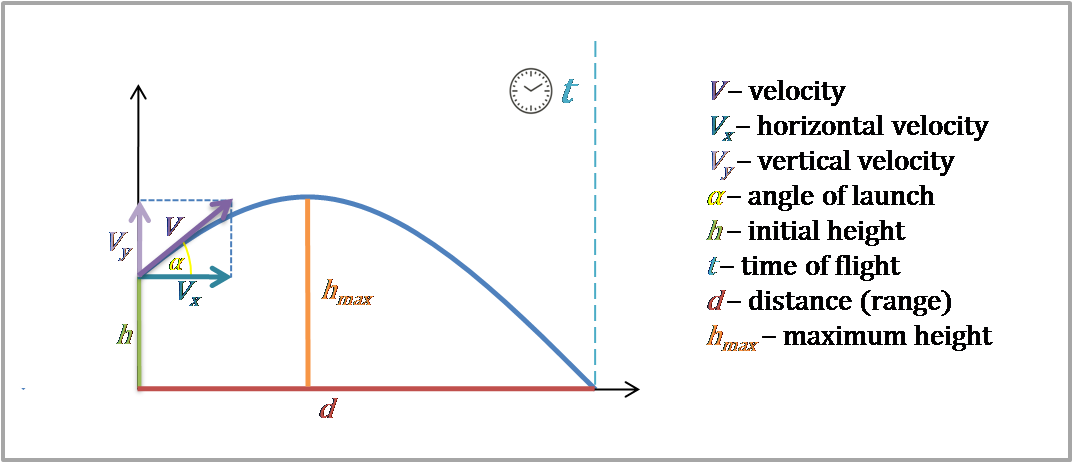
\includegraphics[width=.7\textwidth]{Figures/projectile-motion.png}
            \caption{Throwing a ball as an example of needing initial data.}
            \label{fig:proj_motion}
        \end{figure}
        \noindent We call these values $x(0)$ and $x'(0)$ the \emph{initial data}. 
        
        \begin{df}{Initial Data}{df: initial_data}
            The \boldgreen{initial data} \index{initial data} to an $n$th order ODE are the specific values for
            \[
            x(0),~ x'(0),\dots,~ x^{(n-1)}(0),
            \]
            where $x^{(k)}$ represents the $k$th derivative of $x(t)$.
        \end{df}
        
        \noindent It is from this initial data that we can figure out what a \emph{particular solution} to a problem should be.  Up to this point, we have found a general solution which is really a family of solutions. For real problems, we need one answer and not infinitely many.  
        
        \begin{df}{Particular Solution}{particular_solution}\index{particular solution}
            A \boldgreen{particular solution} is one member of the family of general solutions.  That is, a solution where the constants $c_1,~c_2,\dots,~c_n$ are all uniquely determined.
        \end{df}
        
        \noindent In other words, the particular solution is a single solution to a problem.  Specifically, we call this type of problem where we have initial data present a \boldgreen{initial value problem} \index{initial value problem}.  We will want to make note of this name as we will see \emph{boundary value problems} later on. 
        
        \begin{prop}{Initial Data and Particular Solutions}{initial_data_part_solns}
        In order to find a particular solution to an $n$th order ODE, one needs to know the initial values of the function, its derivative, its second derivative, and all derivatives up to the $(n-1)th$ derivative
        \[
        x(0),~ x'(0),\dots,~ x^{(n-1)}(0).
        \]
        \end{prop}
        
        \noindent Now, let us work through this a bit.  We can set up an initial value problem and from a general solution we can narrow in on a particular solution.  Try to keep in mind what the initial data is really meaning based on the analogy given before.
        
        
        \begin{ex}{Particular Solution to Harmonic Oscillator}{part_soln_harm_osc}
        Consider 
        \[
        u''(t)=-u(t)
        \]
        with initial data
        \[
        u(0)=1, ~ u'(0)=0.
        \]
        This has the general solution
        \[
        u(t)=Ae^{it}.
        \]
        We can find the particular solution by rewriting $x$ slightly using Euler's formula. In particular, we find
        \[
        u(t)=a\cos(t)+ib\sin(t)
        \]
        since $A$ could be any complex number.  You could also not make this substitution and find what complex number $A$ has to be.
        \[
        u(0)=a\cos(0)+ib\sin(0)=1
        \]
        from our initial data.  Specifically, this gives us that
        \[
        a=
        \]
        Then note we also have
        \[
        u'(0)=-a\sin (0) +i b\cos (0)=0
        \]
        which gives us that
        \[
        ib=0 \quad \implies \quad b=0.
        \]
        So our particular solution is
        \[
        u(t)=\cos (t).
        \]
        \end{ex}
        
        \begin{exercise}
        Plot the solution. Can you determine what is happening if we think of the oscillator as a spring mass system? What does the initial data tell us about the spring and mass at the start?
        \end{exercise}
        
        \begin{exercise}
            Instead of making the substitution using Euler's formula, solve for the complex number $A$ that shows up in $u(t)=Ae^{it}$.
        \end{exercise}
        
        The reason why we study these differential systems is to make predictions and models.  Given that, our predictions must be sensible. This means if we are given a differential equation and initial data, there should only be one particular solution.  This is known as \boldgreen{determinism}.     Not all systems are deterministic.  But it turns out the non-deterministic systems are either problematic as models or just very hard to deal with. When solving an ODE, we often call a particular solution a \boldgreen{trajectory}.
        
        \section{Separable Equations}
        The nicest possible ODEs come from equations that are \emph{separable}\index{separable differential equation}.  What this means is that, for example, we have a first order equation like
        \[
        x'=f(t)g(x).
        \]
        Why is this nice? Well, in particular, it means that we can simply integrate this equation to solve it.  Many systems exhibit symmetry that allows for this type of separation, so this technique is crucial.
        
        In general, we have
        \[
        x'=\frac{dx}{dt}
        \]
        and we put
        \begin{align*}
            \frac{dx}{dt}&=f(t)g(x)\\
            \iff \frac{dx}{g(x)} &= f(t)dt.
        \end{align*}
        With this, we can integrate both sides, then solve for $x$. That is, we compute
        \[
        \int \frac{dx}{g(x)} = \int f(t)dt,
        \]
        and we will have an equation where we can isolate $x$
        
        \begin{ex}{Separable ODE}{separable}
        Consider the following ODE where we are trying to find $x(t)$ that solves
        \[
        x'=\frac{t}{x}. 
        \]
        Then we can put
        \begin{align*}
            \frac{dx}{dt}&= \frac{t}{x}\\
            \iff xdx &= t dt.
        \end{align*}
        Then we can take the antiderivative of both sides and find
        \begin{align*}
            \int xdx &= \int t dt\\
            \iff \frac{1}{2}x^2 &= \frac{1}{2}t^2 + c\\
            \iff x&=\sqrt{t^2+2c}.
        \end{align*}
        So now we can verify that this is in fact a solution to our ODE.  So we take
        \[
        x'(t) = \frac{d}{dt}\sqrt{t^2+2c}= \frac{t}{\sqrt{t^2+2c}} = \frac{t}{x}.
        \]
        \end{ex}
        
        \begin{exercise}
        Solve the following ODE using separation
        \[
        x'(t)=t.
        \]
        Note that there will be an undetermined constant that we will learn how to handle next.
        \end{exercise}
        
        \section{Changing Variables and Symmetry}
        
        When presented with a differential equation, it can often be in a form that is not the easiest to work with.  Of course, if you do your modelling step correctly you will end up with a meaningful equation.  We want to be able to translate the correct model equation into one that is more workable.  
        
        We found that separable equations were not too bad to solve as we really just need to integrate.  Now, is it possible to turn an equation into a one that is separable? It turns out, we can when the equation satisfies a certain symmetry condition.  
        
        \begin{prop}{Reduction to Separable Equations}{reduction_separable}
            Consider the first order equation
            \[
            x'=f(x,t).
            \]
            If we have that
            \[
            f(x,t)=f(\lambda x, \lambda t)
            \]
            for any number (or function) $\lambda$, then we can reduce the equation to a separable one by defining a new variable $u=\frac{x}{t}$.
        \end{prop}
        
        The idea of changing variables is immensely important in solving real world problems.  Often times, one can gain insight on the question at hand by searching for these ``better" variables to work in.  
        
        \begin{ex}{Reduction to Separable}{reduction_separable_ex}
            Consider the differential equation
            \[
            x'=\frac{x^2+t^2}{xt}.
            \]
            We can then define
            \[
            f(x,t)=\frac{x^2+t^2}{xt}.
            \]
            Now, we can check that $f(x,t)=f(\lambda x, \lambda t)$ for any $\lambda$ by plugging in.  We have
            \begin{align*}
            f(\lambda x, \lambda t) &= \frac{(\lambda x)^2+(\lambda t)^2}{(\lambda x)(\lambda t)}\\
            &= \frac{\lambda^2(x^2+t^2)}{\lambda^2 xt}\\
            &= \frac{x^2+t^2}{xt}\\
            &=f(x,t).
            \end{align*}
            So our differential equation satisfies the necessary symmetry condition.  So, we can let $u=\frac{x}{t}$ which also means that $x=tu$ and hence
            \[
            f(x,t)=f(tu,t)=\frac{t^2u^2+t^2}{ut^2}=\frac{u^2+1}{u}.
            \]
            Note that given $x=tu$ we have $x'=u+tu'$ which we can now plug into our original expression
            \[
            x'=f(x,t)
            \]
            to get
            \[
            u+tu'=\frac{u^2+1}{u}.
            \]
            Then we can rearrange to isolate $u'$ on the right hand side
            \begin{align*}
                u+tu'&=\frac{u^2+1}{u}\\
                tu'&= \frac{u^2+1}{u}-u\\
                u'&= \frac{1}{tu}.
            \end{align*}
            This is now a separable equation! So, we can solve this in the typical way by noting we have $u'=\frac{du}{dt}$ and putting
            \[
            udu=\frac{dt}{t}.
            \]
            Then we can integrate and solve for $u$
            \begin{align*}
                \int udu &= \int \frac{dt}{t}\\
                \frac{1}{2}u^2 &= \ln(t)+c\\
                u^2&= 2\ln(t)+2c\\
                u&=\pm \sqrt{2\ln(t)+2c}.
            \end{align*}
            Recall that $u=\frac{x}{t}$ and so we have
            \begin{align*}
                \frac{x}{t}&= \pm \sqrt{2\ln(t)+2c}\\
                x&= \pm t\sqrt{2\ln(t)+2c}.
            \end{align*}
            This $x$ is our general solution to the original problem.
        \end{ex}
        
        \newpage
        
        In physical systems that conserve some quantity in time (typically energy), we will see that the differential equations assume a certain form.  This form is of an \emph{autonomous} differential equation.
        
        \begin{df}{Autonomous ODE}{autonomous_ode}
            A first order differential equation is \boldgreen{autonomous}\index{autonomous differential equation} if it can assume the form
            \[
            x'=f(x).
            \]
        \end{df}
        \noindent A first order autonomous equation is also separable. So there is not much more here to say.  They do show up quite often.
        
        Another way that symmetry can help us is more from a modelling perspective. For example, it is possible to make more clever measurements of your system! This is a much needed tool for someone keen on doing experiments. For now, do your best to follow the logic of the following substitution.  This is an example of how one can view a problem in a new way and make it easier.  We should all love symmetry like this! 
        
        \begin{ex}{Changing Variables in Harmonic Oscillator}{changing_var_harmonic}
        Consider the harmonic oscillator equation given by
        \[
        y'' = -\frac{k}{m}(y(t)-L).
        \]
        This equation, being second order, is immediately more difficult to solve.  What we can do, however, is make a change of variables to
        \[
        x(t)=y(t)-L
        \]
        and note that
        \[
        x''(t)=y''(t)
        \]
        but the ODE changes to
        \[
        x''(t)=\frac{k}{m}x(t).
        \]
        This is much easier to solve.  The idea of changing variables is extremely helpful.
        
        In these new variables, we can see the following figure.
        \begin{figure}[H]
            \centering
            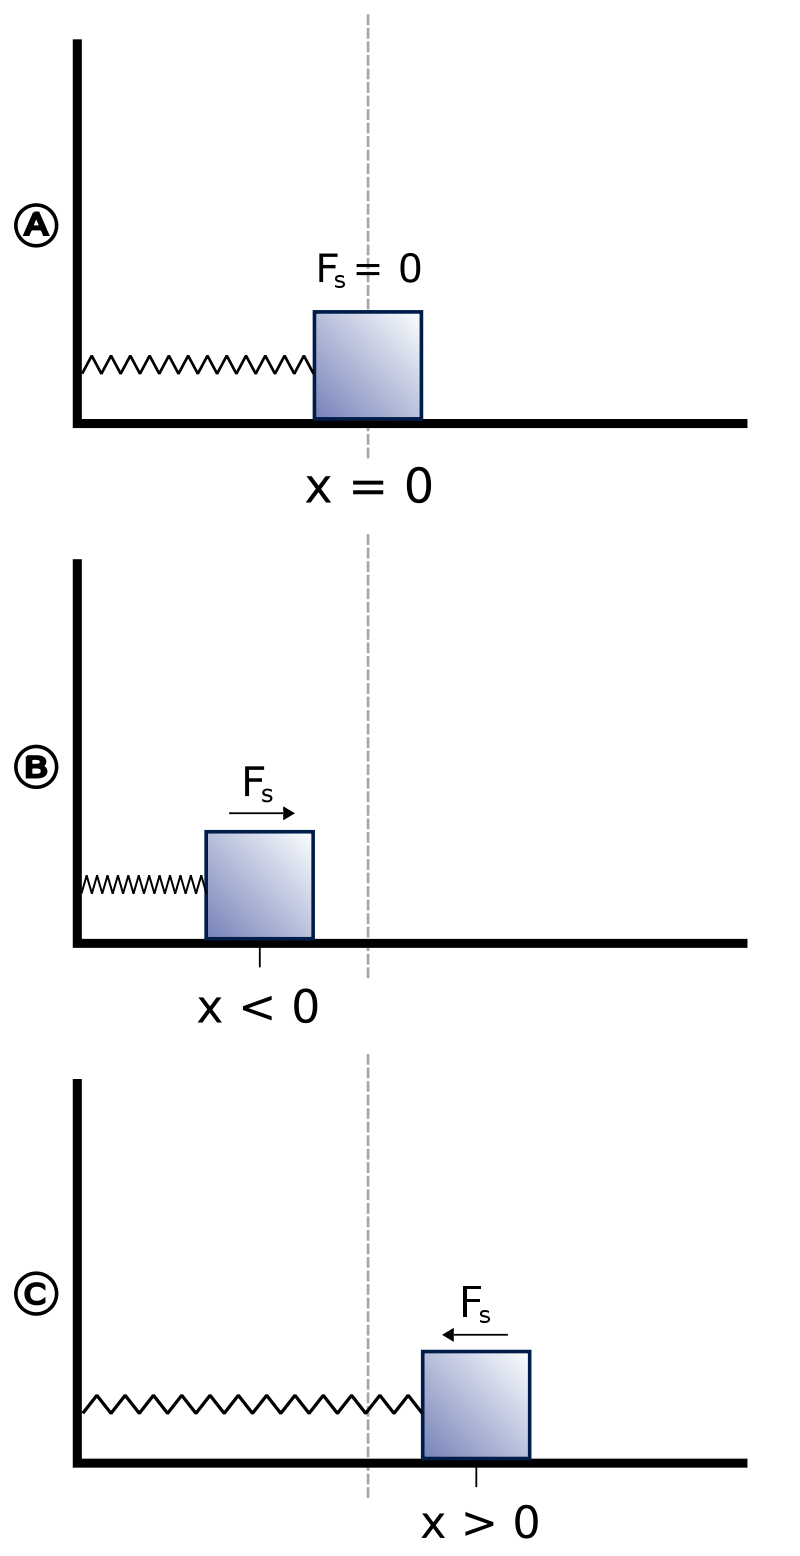
\includegraphics[width=.3\textwidth]{Figures/spring-mass.png}
            \caption{Spring-Mass system in the new variables. The dashed line represents the rest length $L$.}
            \label{fig:spring_mass}
        \end{figure}
        Interestingly enough, the rest length $L$ does not enter the new equation now. As it turns out, it is essentially a useless parameter for understanding the problem.  However, an engineer would care about changing back to our original variable $y$ as the length of a spring factors into design!
        
        How could you know to make this change? Two ways.  First, one can observe how a spring mass system oscillates.  Set up the experiment and watch for yourself, if you'd like.  What you'll see is that the mass oscillates in a symmetric way about the rest length of the spring. The experimentalist mindset will then suggest that you make the measurement about this position! The other way to observe this is as a mathematician would.  In our original expression you can notice that we have $y(t)-L$ as a quantity and that 
        \[
        \frac{d}{dt} (y(t)-L) = y'(t).
        \]
        This may be less intuitive to see, but this tells us that we can safely exchange the quantity $y(t)-L$ for a new quantity $x(t).$
        \end{ex}
        
        Earlier I claimed that this simplified equation
        \[
        x'' = -\frac{k}{m}x
        \]
        is equivalent to
        \[
        u''=-u
        \]
        by changing the units in which we measure the problem.  Indeed, consider the change of variables
        \[
        u(t)=x\left( \sqrt{k}{m}\right).
        \]
        Then 
        \[
        u'(t)=\sqrt{k}{m}x\left(\sqrt{k}{m}\right) \qquad \textrm{and} \qquad u''(t)=\frac{k}{m}x\left( \sqrt{k}{m}\right).
        \]
        
        \begin{exercise}
        Using the substitution shown above, show that the equation
        \[
        x'' = -\frac{k}{m}x
        \]
        is equivalent to
        \[
        u''=-u.
        \]
        \end{exercise}
        
        \section{First Order Linear Differential Equations}
        
        Another nice set of equations that we can solve come in the form of linear equations.  In particular, we first consider \emph{first order linear ODEs}\index{linear differential equation} but will later consider the second order version as well.  Generally, linear problems tend to be solvable whereas nonlinear problems are very hard.  One can also learn how to approximate nonlinear problems via linearization, but we do not do that here.
        
        \begin{df}{First Order Linear ODE}{first_order_lin}
            A \boldgreen{first order linear ODE} is an equation that can assume the form
            \[
            x'+f(t)x=g(t).
            \]
        \end{df}
        
        There is a general technique for solving this type of equation and, in fact, a general technique for solving higher order linear equations.  More on that later.  For now, let us work to solve this problem.  The method we will use utilizes a function called an \boldgreen{integrating factor}\index{integrating factor}. The idea is that we can use the format of the equation to our advantage.
        
        \subsubsection{Integrating Factor}
        Consider a first order linear ODE given by
        \[
        x'+f(t)x=g(t).
        \]
        Then, multiply the whole expression by a yet undetermined function $\mu(t)$ to get
        \begin{equation}
        \mu(t)x'+\mu(t)f(t)x=\mu(t)g(t). \label{eq:int_fact_1}
        \end{equation}
        The reason we have done this is that we can now take a look at the derivative of the product
        \begin{equation}
        \left( \mu(t)x\right)'= \mu'(t)x+\mu x'. \label{eq:int_fact_2}
        \end{equation}

        From here, we can set this product derivative (right hand side of \ref{eq:int_fact_2}) equals the left hand side of expression \ref{eq:int_fact_1}.  This gives us
        \[
        \mu'(t)x+\mu x' = \mu(t)x'+\mu(t) f(t) x
        \]
        which means that
        \[
        \mu'(t)x=\mu(t) f(t) x.
        \]
        This is a separable ODE! So we can solve this for $\mu$ using the separation technique. This $\mu$ is the integrating factor.
        
        \begin{exercise}
            Solve the separable ODE
            \[
            \mu'(t)x=\mu(t)f(t)x
            \]
            for $\mu$ and show that you find
            \[
            \mu(t) = e^{\int f(t)dt}.
            \]
        \end{exercise}
        
        \noindent From the exercise, we have that
        \[
        \mu(t)=e^{\int f(t)dt}
        \]
        and we can use this to complete the problem.  Specifically, we have that the left hand side of \ref{eq:int_fact_2} is equal to the right hand side of \ref{eq:int_fact_1} to get
        \[
        (\mu(t) x)' = \mu(t)g(t).
        \]
        We can integrate both sides and solve for $x$ to find
        \[
        \boxed{x = \frac{1}{\mu(t)}\int \mu(t) g(t)dt.}
        \]
        The above expression for $x$ tells us the general solution to any first order linear ODE.
        
        \begin{ex}{Solving an ODE with Integrating Factor}{solving_ode_int_fact}
            Consider the first order equation
            \[
            x'+\frac{2x}{t}=2\cos(t).
            \]
            Note that we can say $f(t)=\frac{2}{t}$ and then 
            \begin{align*}
            \mu(t)&=e^{\int \frac{2}{t}dt}\\
            &= e^{2\ln(t)}\\
            &=t^2.
            \end{align*}
            Note, when computing the integrating factor $\mu$ we do not need to have a $+c$ after integrating. It will cancel later on if you do include it. Next, we note that
            \[
            x=\frac{1}{\mu(t)} \int \mu(t) g(t)dt
            \]
            where $g(t)=2\cos(t)$ in this case.  Thus
            \begin{align*}
                x&=\frac{1}{t^2} \int t^2 \cdot 2\cos(t)dt\\
                &=\frac{2}{t^2} \left(t^2\sin(t)+2t\cos(t)-2\sin(t)+c\right),
            \end{align*}
            where the last equality involved using integration by parts twice.  So we have found a general solution to our original ODE.
        \end{ex}
        
        \begin{exercise}
            Complete the integration by parts in the above example.
        \end{exercise}
        
        Just to introduce some terminology, we can note that if we have a first order linear ODE of the form
        \[
        x'+f(t)x=0
        \]
        we call this equation \boldgreen{homogeneous}\index{homogeneous!differential equation}.  Otherwise, we have that the expression with a nonzero right hand side
        \[
        x'+ f(t)x=g(t)
        \]
        is called \boldgreen{inhomogenous}\index{inhomogeneous!differential equation}.  The homogeneous case for first order equations are simply separable equations and the distinction here is not really necessary.
        
        \section{Applications to Chemical Kinetics}
        \index{chemical kinetics}
        As a chemist, one would probably like to understand how we can model elementary chemical reactions with mathematics.  For example, maybe we would like to understand the rate of reaction of hydrogen $H_2$ and oxygen $O_2$ to create water $H_2 O$. We typically write
        \[
        2H_2 + O_2 \to 2H_2O.
        \]
        \noindent Of course, we should actually be writing
        \[
        2H_2 + O_2 \leftrightarrows 2H_2O
        \]
        since real reactions have an equilibrium.  The amount of back and forth in a reaction also depends on parameters like temperature, pressure, or concentration.
        
        For now, let us assume we are looking at the original model which can we written as a sum of $m$ reactants $R_i$ each with an amount $r_i$ that give us an amount $p_i$ of $n$ different products $P_j$. That is, we have a reaction
        \begin{align*}
            r_1R_1 + r_2R_2 + \cdots + r_mR_m \to p_1 P_1 + p_2P_2 +\cdots p_n P_n,
        \end{align*}
        that gives us an equation
        \[
        \sum_{i=1}^m r_iR_i = \sum_{j=1}^n p_jP_j.
        \]
        The second is just a mathematically succinct way of representing the quantitites in the reaction. We will call the $r_i$ and $p_j$ the \boldgreen{stoichiometric variables}. We often write the equation above in the following form:
        \begin{equation}
        0=\sum_{j=1}^n p_j P_j - \sum_{i=1}^m r_iR_i. \label{eq:stoich}
        \end{equation}
        
        Suppose we start with an initial amount of substance $A$, $N_{A0}$. Then we say that the amount of species $A$ at time $t$ is $N_{A}$.  The amount of reaction observed is given by the \boldgreen{extent of reaction} $\xi$ defined by
        \[
        N_A = N_{A0}+a\xi.
        \]
        Note that $a$ will be negative for products as the number of products decreases over time. To see this, see \ref{eq:stoich} which states that the total number of species has to be conserved. Then the \boldgreen{rate of conversion} is 
        \begin{align*}
            \rho &= \frac{d\xi}{dt}\\
            &= \frac{1}{a}\frac{dN_a}{dt}.
        \end{align*}
        
        More often than not, we care about concentrations of chemicals as opposed to amount. So we let
        \[
        [A]=\frac{N_A}{V}
        \]
        where $V$ is the volume the substance $A$ is contained in.  Then we have
        \[
        v=\frac{\rho}{V}=\frac{1}{a}\frac{d[A]}{dt}.
        \]
        Now, for a reaction 
        \[
        r_1R_1 + r_2R_2 + \cdots + r_mR_m \to p_1 P_1 + p_2P_2 +\cdots p_n P_n,
        \]
        we must have that the concentrations must change with matching rates so that
        \[
        v=-\frac{1}{r_i}\frac{d[R_i]}{dt}=\frac{1}{p_j}\frac{d[P_j]}{dt},
        \]
        for every product $P_j$ and reactant $R_i$.
        
        \begin{ex}{$H_2$ and $O_2$ to $H_2O$}{water}
        If we are wishing to model
        \[
        2H_2 + O_2 \to 2H_2O
        \]
        we will have the equations
        \begin{align*}
            v=-\frac{1}{2}\frac{d[H_2]}{dt}=-\frac{d[O_2]}{dt}=\frac{1}{2}\frac{d[H_2O]}{dt}.
        \end{align*}
        \end{ex}
        
        From experiment one can determine that
        \[
        v=k[R_1]^{\alpha_1}[R_2]^{\alpha_2}\cdots
        \]
        which allows us to complete our model.  We call $k$ the \boldgreen{rate constant} of the reaction and the numbers $\alpha_i$ dtermine that \boldgreen{order of the reaction}. We say that $\alpha_i$ is the order with respect to the reactant $R_i$. For example, we may have
        \begin{itemize}
            \item First order: $R \to \textrm{Products}$;
            \item Second order: $2R \to \textrm{Products}$;\\
            \item Second order: $R_1+R_2 \to \textrm{Products}$.
        \end{itemize}
        
        \begin{ex}{First Order Reaction}{first_order_react}
        Consider a reaction
        \[
        R \to \textrm{Products}
        \]
        with an initial concentration of $R$ given by $[R]_0$. We then have
        \[
        v=\frac{-d[R]}{dt}=k[R].
        \]
        For ease of notation, let $x=[R]$ and we have
        \[
        x'=-kx,
        \]
        which we have solved before.
        \end{ex}
        
        \begin{exercise}
        Either solve the above differential equation again, or find the solution to the initial value problem somewhere in this text.
        \end{exercise}
        
        \begin{ex}{Second Order Reaction}{second_order_react}
        Consider a reaction
        \[
        2R \to \textrm{Products}
        \]
        with an initial concentration $[R]_0$.  Then we have
        \[
        v=-\frac{1}{2} \frac{d[R]}{dt}=k[R]^2.
        \]
        Again, let $x=[R]$ and we have the ODE
        \[
        x'=-2kx^2.
        \]
        \end{ex}
        
        \begin{exercise}
        Find the particular solution to the initial value problem posed in the previous example.
        \end{exercise}
        
        
        %% THERE MAY BE MISTAKES HERE
        \begin{ex}{Several Reactions}{sev_react}
        Consider a chain of reactions as follows
        \[
        A\xrightarrow{k_1} B \xrightarrow{k_2} C.
        \]
        Then we wish to describe the concentrations of each species $A$, $B$, and $C$ over time. We know that we have
        \[
        \frac{d[A]}{dt}=-k_1[A]
        \]
        and it follows that
        \[
        \frac{d[b]}{dt}=k_1[A]-k_2[B].
        \]
        Then, at time $t=0$ we have initial concentrations $[A]_0$, $[B]_0=0$, and $[C]_0$ so that we are only starting with species $A$. Later on, at time $t$, we have $[A]=[A]-x$ and $[B]=y$ which means that we have $[C]=x-y$.  Note that $[C]$ is created by $A\to B$ and from $B\to C$ so we must subtract off the concentration of $B$ that has not converted to species $C$ yet. This gives us the equations
        \begin{equation}
                        \frac{d([A]_0-x)}{dt}=-k_1([A]-x) \label{eq:chem_a}
        \end{equation}
        \begin{equation}
                        \frac{dy}{dt}=k_1([A]_0-x)-k_2y. \label{eq:chem_b}
        \end{equation}
        Note that \ref{eq:chem_a} is a separable equation with solution
        \[
        [A]_0-x=[A]_0e^{-k_1t}.
        \]
        We can then substitute in this solution to \ref{eq:chem_b} to get
        \[
        \frac{dy}{dt}=[A]_0k_1e^{-k_1t}-k_2y
        \]
        which gives us the first order linear equation
        \[
        y'+k_2y=[A]_0k_1e^{-k_1t}.
        \]
        To solve this, we find the integrating factor
        \[
        \mu(t)=e^{\int k_2 dt}=e^{k_2t}.
        \]
        Then we have that
        \[
        y=\frac{1}{e^{k_2t}}\int e^{k_2t}[A]_0k_1e^{-k_1t}dt=[A]_0k_1e^{-k_2t}\int e^{(k_2-k_1)t}dt.
        \]
        This integral comes down to two cases; first when $k_1=k_2$ and when $k_1\neq k_2$. Thus we have
        \[
        y=\begin{cases}
        \frac{[A]_0k_1}{k_2-k_1}e^{-k_1t}+ce^{-k_2t} & k_1\neq k_2\\
        [A]_0k_1te^{-k_1t}+ce^{-k_2t} & k_1=k_2.
        \end{cases}
        \]
        Using our initial conditions, we have $y=0$ at time $t=0$ which gives us the particular solution
        \[
        y=\begin{cases}
        \frac{[A]_0k_1}{k_2-k_1}\left( e^{-k_1t}-e^{-k_2t}\right) & k_1\neq k_2\\
        [A]_0k_1te^{-k_2t} & k_1=k_2.
        \end{cases}
        \]
        
        Now, we will have that each concentration can be written as
        \begin{align*}
            [A]&=[A]_0e^{-k_1t}\\
            [B]&=\begin{cases}
        \frac{[A]_0k_1}{k_2-k_1}\left( e^{-k_1t}-e^{-k_2t}\right) & k_1\neq k_2\\
        [A]_0k_1te^{-k_2t} & k_1=k_2.
        \end{cases}\\
        [C]&=[A]_0-[A]-[B].
        \end{align*}
        Now, we can plot the concentrations below letting $[A]$ be in purple, $[B]$ in red, and $[C]$ in black.
        \begin{figure}[H]
    \centering
    \begin{subfigure}[h]{0.3\textwidth}
        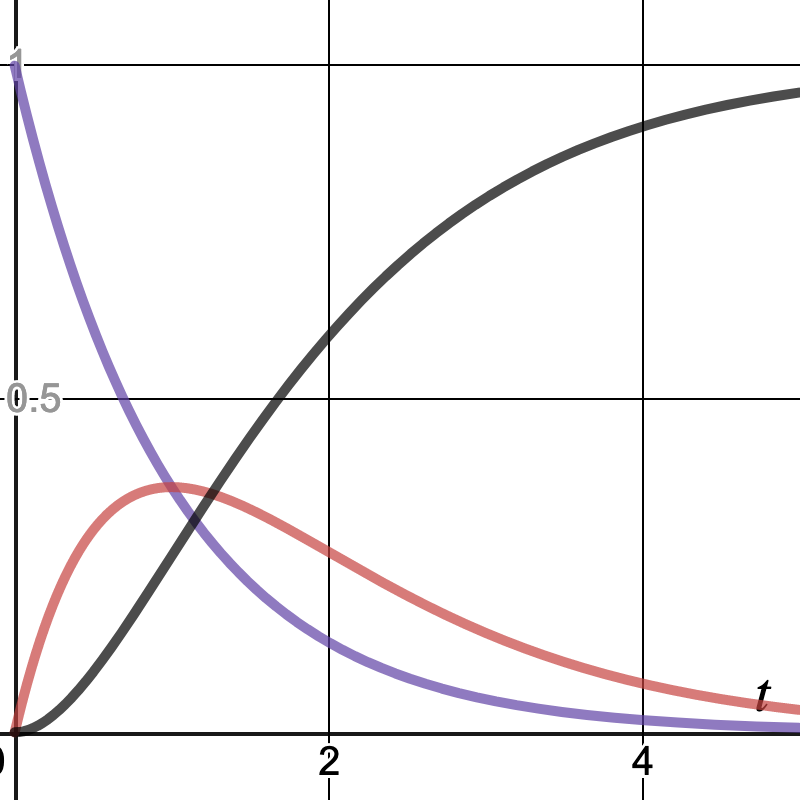
\includegraphics[width=\textwidth]{Figures_Part_2/k1=k2.png}
        \caption{$k_1=k_2=1$.}
    \end{subfigure}
    ~ 
    \begin{subfigure}[h]{0.3\textwidth}
        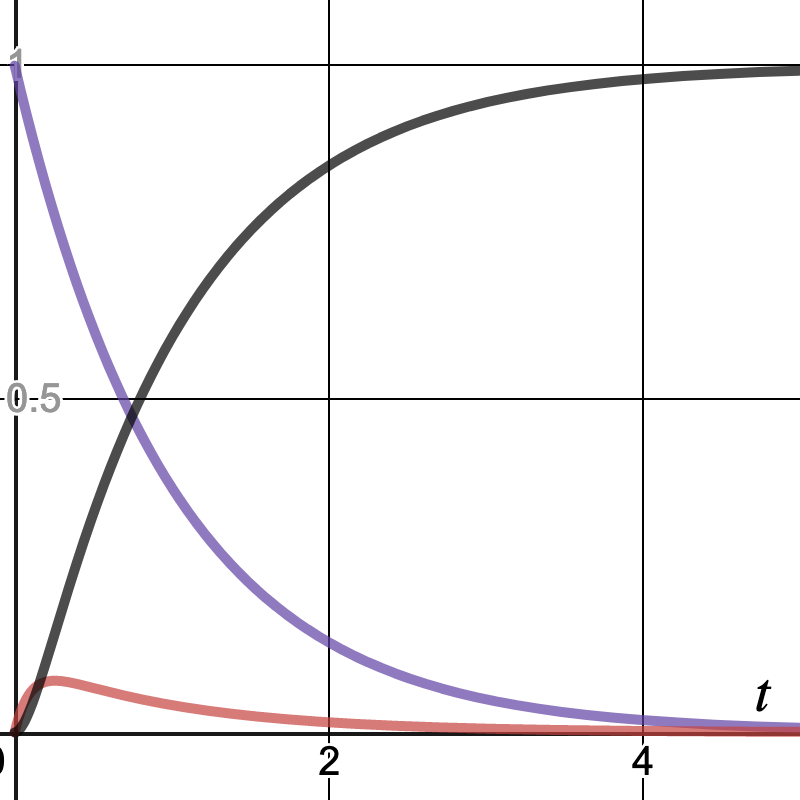
\includegraphics[width=\textwidth]{Figures_Part_2/k1=1k2=10.png}
        \caption{$k_1=1$ and $k_2=10$.}
    \end{subfigure}
    ~
    \begin{subfigure}[h]{0.3\textwidth}
        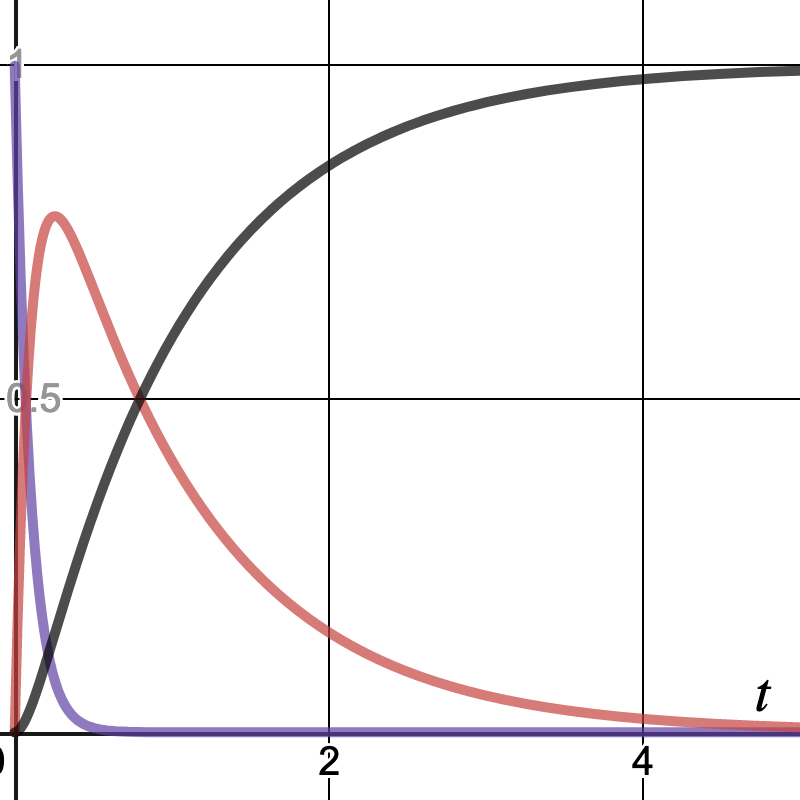
\includegraphics[width=\textwidth]{Figures_Part_2/k1=10k2=1.png}
        \caption{$k_1=10$ and $k_2=1$.}
    \end{subfigure}

        \end{figure}
        \end{ex}
        
        \begin{exercise}
        Go through the previous example and fill in the missing steps.
        \end{exercise}
        
        \section{Second Order Equations}
        
        Since Newtonian physics is governed by the equation
        \[
        F=ma=mx''
        \]
        we often see differential equations that are second order.  The question is then, how can we solve these?  
        
        There are a two main forms of second order equations we will consider, but there are more out there. Let's define the class of equations we will stick with.
        
        \begin{df}{Second Order Linear ODEs}{second_order_lin}
            A second order ODE is \boldgreen{linear}\index{linear!differential equation} if it can assume the form 
            \[
            x''+f(t)x'+g(t)x=h(t).
            \]
            We say that the equation is \boldgreen{homogeneous}\index{homogeneous!differential equation} if $h(t)=0$ and otherwise it is \boldgreen{inhomogenous}\index{inhomogeneous!differential equation}.
        \end{df}
        
        \begin{remark}
        An inhomogenous second order linear ODE \underline{can} be always be solved with the functions $f$, $g$, and $h$ are smooth enough.  We will not cover solving this general of a problem here.
        \end{remark}
        
        \subsection{Homogeneous and Constant Coefficients}
        Specifically, we care about homogeneous second order linear ODEs where the functions $f(t)=b$ and $g(t)=c$ are constant.  These will be the most simple to solve yet fairly applicable. An equation like this can be rearranged to take the form
        \[
        x''+bx'+cx=0.
        \]
        A reasonable guess (or \boldgreen{ansatz}\index{ansatz}) for a solution is an exponential function of the form
        \[
        x(t)=Ae^{\lambda t}
        \]
        where $A$ is an arbitrary constant. Since we can see that each successive derivative seems to only multiply our function by a constant, this is a good first guess. If we try to make this function $x$ work to solve our ODE, we plug it in and see that we get
        \begin{align*}
            \left(Ae^{\lambda t}\right)''+b\left(Ae^{\lambda t}\right)'+cAe^{\lambda t}&=0\\
            \iff\lambda^2 Ae^{\lambda t}+\lambda b Ae^{\lambda t} +c Ae^{\lambda t}&=0\\
            \iff Ae^{\lambda t}\left( \lambda^2 + b\lambda +c\right)&=0\\
            \iff \lambda^2 +b\lambda +c &=0.
        \end{align*}
        The last equality must be true since $Ae^{\lambda t}$ is never equal to zero.  Thus, it seems we found a solution to the equation via the roots of this polynomial
        \[
        \lambda^2+b\lambda +c,
        \]
        which we will refer to as the \boldgreen{characteristic polynomial}\index{characteristic polynomial}. The roots of the characteristic polynomial are then able to be found with the quadratic formula to yield
        \[
        \lambda=\frac{-b\pm \sqrt{b^2-4c}}{2}.
        \]
        This leads us to the following.
        
        \begin{prop}{Solutions to Linear Constant Coefficient Second Order ODE}{solutions_hom_constant}
        Given the differential equation
        \[
        x''+bx'+cx=0
        \]
        with roots of the characteristic polynomial
        \[
        \lambda^2+b\lambda +c
        \]
        equal to $\lambda_1$ and $\lambda_2$, we have the general solution:
        \[
        x(t)=C_1 e^{\lambda_1t}+C_2e^{\lambda_2t}
        \]
        where $C_1,C_2,\lambda_1,\lambda_2 \in \C$.
        \end{prop}
        
        \begin{question}
        Above we see that we have a sum of solutions and our ansatz only chose one. Is it always possible to have a sum of different solutions be a solution?
        \end{question}
        
        \begin{answer}
        Yes. We will see by the following theorem that this is the case! This is an important result for studying quantum systems.
        \end{answer}
        
        \begin{thm}{Superposition of Solutions}{superposition_solns}
        Let $x_1$ and $x_2$ be general solutions to the equation
        \[
        x''+f(t)x'+g(t)x=0.
        \]
        Then any \boldgreen{linear combination}\index{linear combination} (or \boldgreen{superposition}\index{superposition}) of solutions
        \[
        \alpha_1 x_1 + \alpha_2 x_2
        \]
        with $\alpha_1,\alpha_2\in \C$, is also a solution.\\
        
        \begin{proof}
        Let $x_1$ and $x_2$ be general solutions to the above ODE. Then consider the function
        \[
        x=\alpha_1 x_1 + \alpha_2 x_2.
        \]
        Then we have
        \begin{align*}
            x''+f(t)x'+g(t)x&= (\alpha_1 x_1 + \alpha_2 x_2)''+f(t)(\alpha_1x_1+\alpha_2 x_2)'+g(t)(\alpha_1x_1+\alpha_2x_2)\\
            &= \alpha_1 x_1'' + \alpha_2 x_2'' + \alpha_1 f(t)x'+\alpha_2 f(t)x_2'+\alpha_1 g(t)x_1 + \alpha_2 g(t) x_1\\
            &= \alpha_1 ( x_1''+f(t)x_1'+g(t)x_1)+\alpha_2(x_2''+f(t)x_2'+g(t)x_2)\\
            &=0, \quad\textrm{since $x_1$ and $x_2$ are solutions.}
        \end{align*}
        Hence $x=\alpha_1x_1 + \alpha_2 x_2$ is also a solution.
        \end{proof}
        \end{thm}
        
        \begin{remark}
        You may have heard of superposition in quantum mechanics. It turns out that this is exactly what is meant in the mathematical theory. Eventually, we'll see an example of what this physically means in a quantum system.
        \end{remark}
        
        \begin{ex}{Solving the Harmonic Oscillator}{solve_harmonic}
        Consider the equation
        \[
        mx''=-kx
        \]
        with the initial data $x(0)=1$ and $x'(0)=0$. We have shown that we have a solution to this equation before, but now we can explicitly solve it.  We can rewrite the ODE as a second order linear homogeneous equation with constant coefficients by putting
        \[
        x''+\frac{k}{m}x=0.
        \]
        Then, for sake of notation, let $\omega = \sqrt{\frac{k}{m}}$ so that
        \[
        x''+\omega^2x=0.
        \]
        Then the characteristic polynmomial is
        \[
        \lambda^2+\omega^2
        \]
        and the roots are
        \begin{align*}
            \lambda^2+\omega^2&=0\\
            \lambda^2&=-\omega^2\\
            \iff \lambda&= \pm \sqrt{-\omega^2}= \pm i \omega.
        \end{align*}
        Thus, the general solution is then
        \[
        x=C_1 e^{i\omega t}+C_2e^{-i\omega t}
        \]
        where $C_1,C_2\in \C$.
        
        Now, we can find the particular solution from the initial data $x(0)=1$ and $x'(0)=0$ and letting
        \[
        C_1=a_1+b_1i \qquad \textrm{and} \qquad C_2=a_2+b_2i.
        \]
        We then have
        \begin{align*}
                    1=x(0)&=(a_1+b_1i)e^{i\omega \cdot 0}+(a_2+b_2 i)e^{-i\omega \cdot 0}\\
                    &=(a_1+b_1i)+(a_2+b_2i)\\
                    &=(a_1+a_2)+i(b_1+b_2).
        \end{align*}
        Thus we must have 
        \begin{align*}
            a_1+a_2&=1\\
            b_1+b_2&=0 ~\implies~ b_1=-b_2.
        \end{align*}
        From the other initial condition, we have
        \begin{align*}
        0=x'(0)&=\omega(a_1+b_1i)e^{i\omega \cdot 0}-\omega (a_2+b_2i)e^{i\omega \cdot 0}\\
        &=(a_1-a_2)+i(b_1-b_2).
        \end{align*}
        Thus we have
        \begin{align*}
            a_1-a_2&=0 ~\implies~ a_1=a_2\\
            b_1-b_2&=0 ~\implies~ b_1=b_2.
        \end{align*}
        Now we have $b_1=-b_2$ and $b_1=b_2$ which means $b_1=b_2=0$.  Then, we also have $a_1=a_2$ which we can substitute into $a_1+a_2=1$ to find that $a_1=a_2=1/2$.  Hence we have our particular solution
        \begin{align*}
            x(t)&=\frac{1}{2}e^{i\omega t}+\frac{1}{2}e^{-i\omega t}.
            \end{align*}
            This, we can rewrite to find a more familiar form of the solution by
            \begin{align*}
            x(t)&= \frac{1}{2}(\cos(\omega t)+i\sin(\omega t)) + \frac{1}{2}(\cos(-\omega t)+i\sin(-\omega t))\\
            &= \frac{1}{2}(\cos(\omega t)+i\sin(\omega t))+\frac{1}{2}(\cos(\omega t)-i\sin(\omega t))
            &=\cos(\omega t).
        \end{align*}
        Note that I used the fact that sine is an odd function meaning that $\sin(-x)=-\sin(x)$ and that cosine is an even function meaning $\cos(-x)=\cos(x)$.  
        \end{ex}
        
        \newpage
        
        \begin{exercise}
        Find where we claimed a solution to the harmonic oscillator earlier in this text and check that this solution matches that.
        \end{exercise}
        
        \subsection{Qualitative Analysis}
        
        Solutions to homogeneous second order linear ODEs with constant coefficients only come in a few different classes of solutions. Essentially, they oscillate, exponentially grow or decay, or a combination of the two.  There are some edge cases to be careful of, but they are not typical.  Let's see why this is the case.
        
        Recall that we have, in general, an equation 
        \[
        x''+bx'+cx=0
        \]
        which gives rise to the characteristic polynomial
        \[
        \lambda^2+b\lambda + c.
        \]
        The roots are then
        \[
        \lambda = \frac{-b\pm \sqrt{b^2-4c}}{2}= \frac{-b}{2}\pm \frac{\sqrt{b^2-4c}}{2}.
        \]
        These roots can be real, complex, or purely imaginary. The real part can be greater than zero, or less.  These facts encompass all the solutions we care about.
        
        \begin{itemize}
            \item \textbf{Case 1:} Consider the case where the roots of the characteristic polynomial are both real and denote the roots by $\lambda_1$ and $\lambda_2$.  If this is the case, then we must have that $b^2>4c$ so that the square root in the quadratic formula is not of a negative number. For this, we have two subcases.
            \begin{itemize}
                \item \textbf{Subcase 1:} If we have two distinct real roots, $\lambda_1$ and $\lambda_2$ where $\lambda_1\neq \lambda_2$, then our general solution to the equation is
                \[
                x(t)=C_1e^{\lambda_1 t}+C_2e^{\lambda_2 t}.
                \]
                Note that $\lambda_1$ and $\lambda_2$ could be both positive, both negative, one negative one positive, or either could be zero as well.
                
                Let's say we have $\lambda_1=1$, $\lambda_2=-1$ and let $C_1=C_2=1$. Then the solution plotted in the $xt$-plane looks like
                \begin{figure}[H]
                    \centering
                    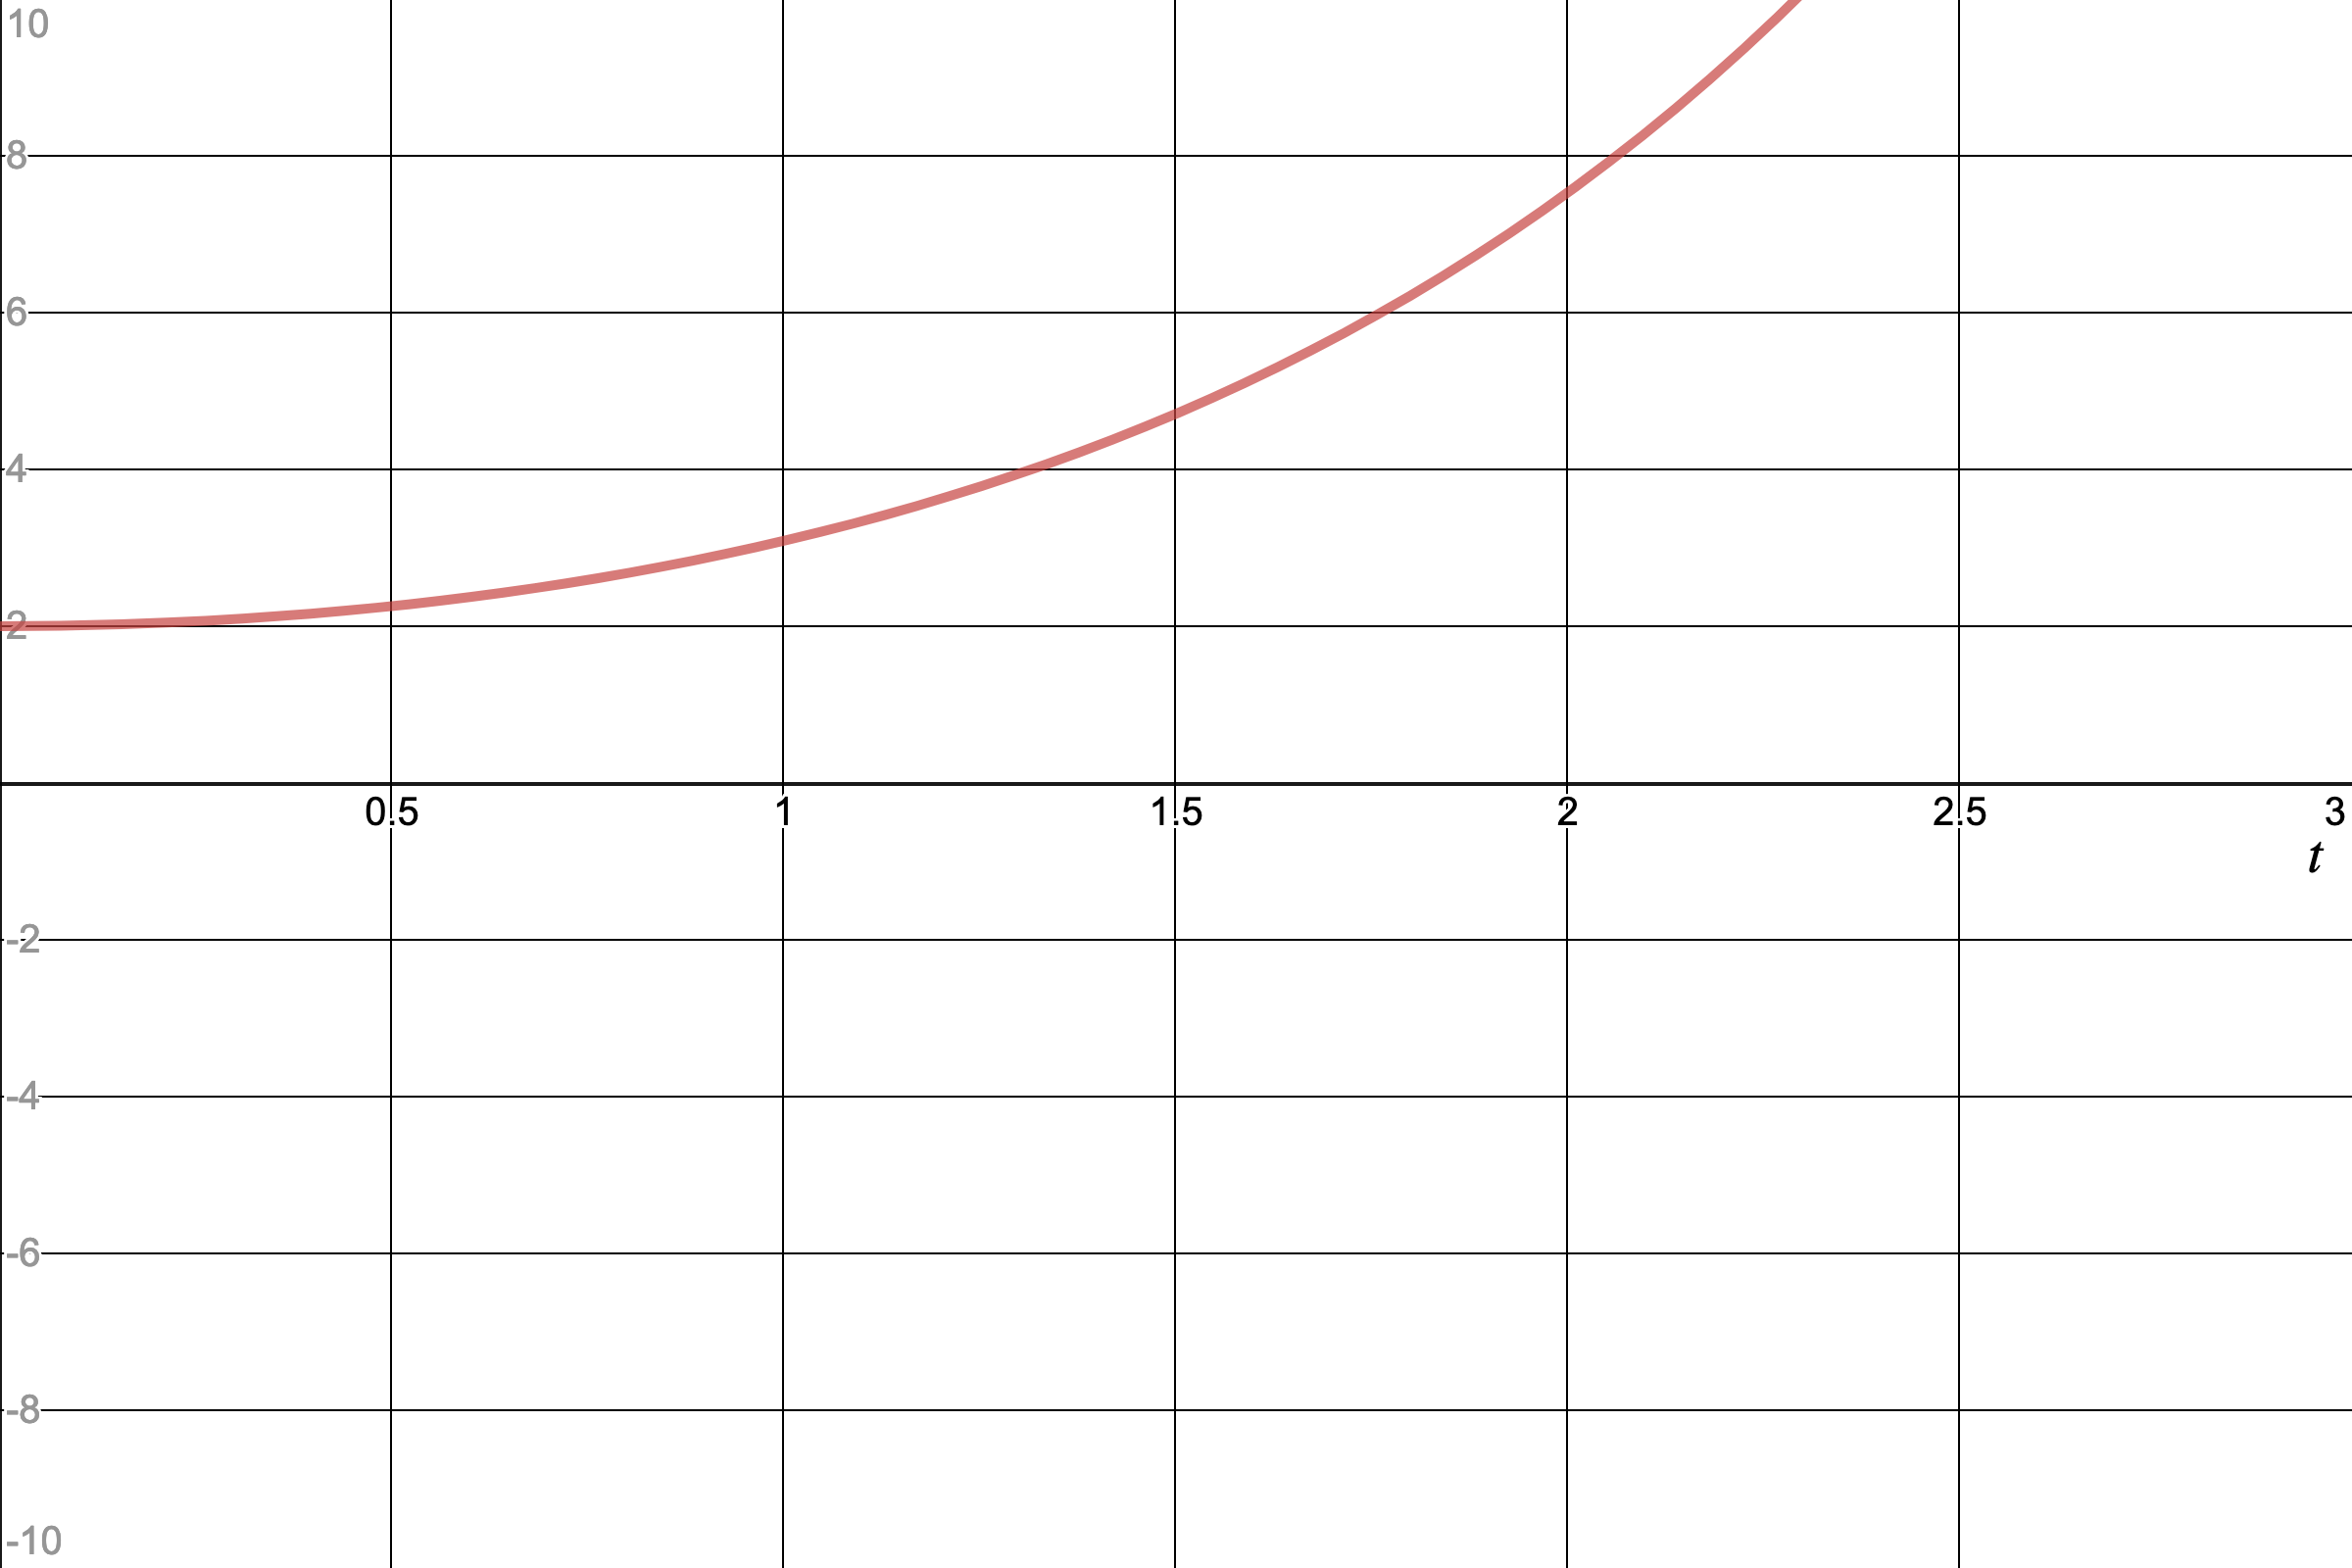
\includegraphics[width=.7\textwidth]{Figures_Part_2/l1=1_l2=-1.png}
                \end{figure}
                \item \textbf{Subcase 2:} If we have two identical real roots, $\lambda=\lambda_1=\lambda_2$ then the general solution is
                \[
                x(t)=C_1 e^{\lambda t}+C_2te^{\lambda t}.
                \]
                
                Here, we can take $\lambda=1$ and let $C_1=C_2=1$ and plot the solution:
                \begin{figure}[H]
                    \centering
                    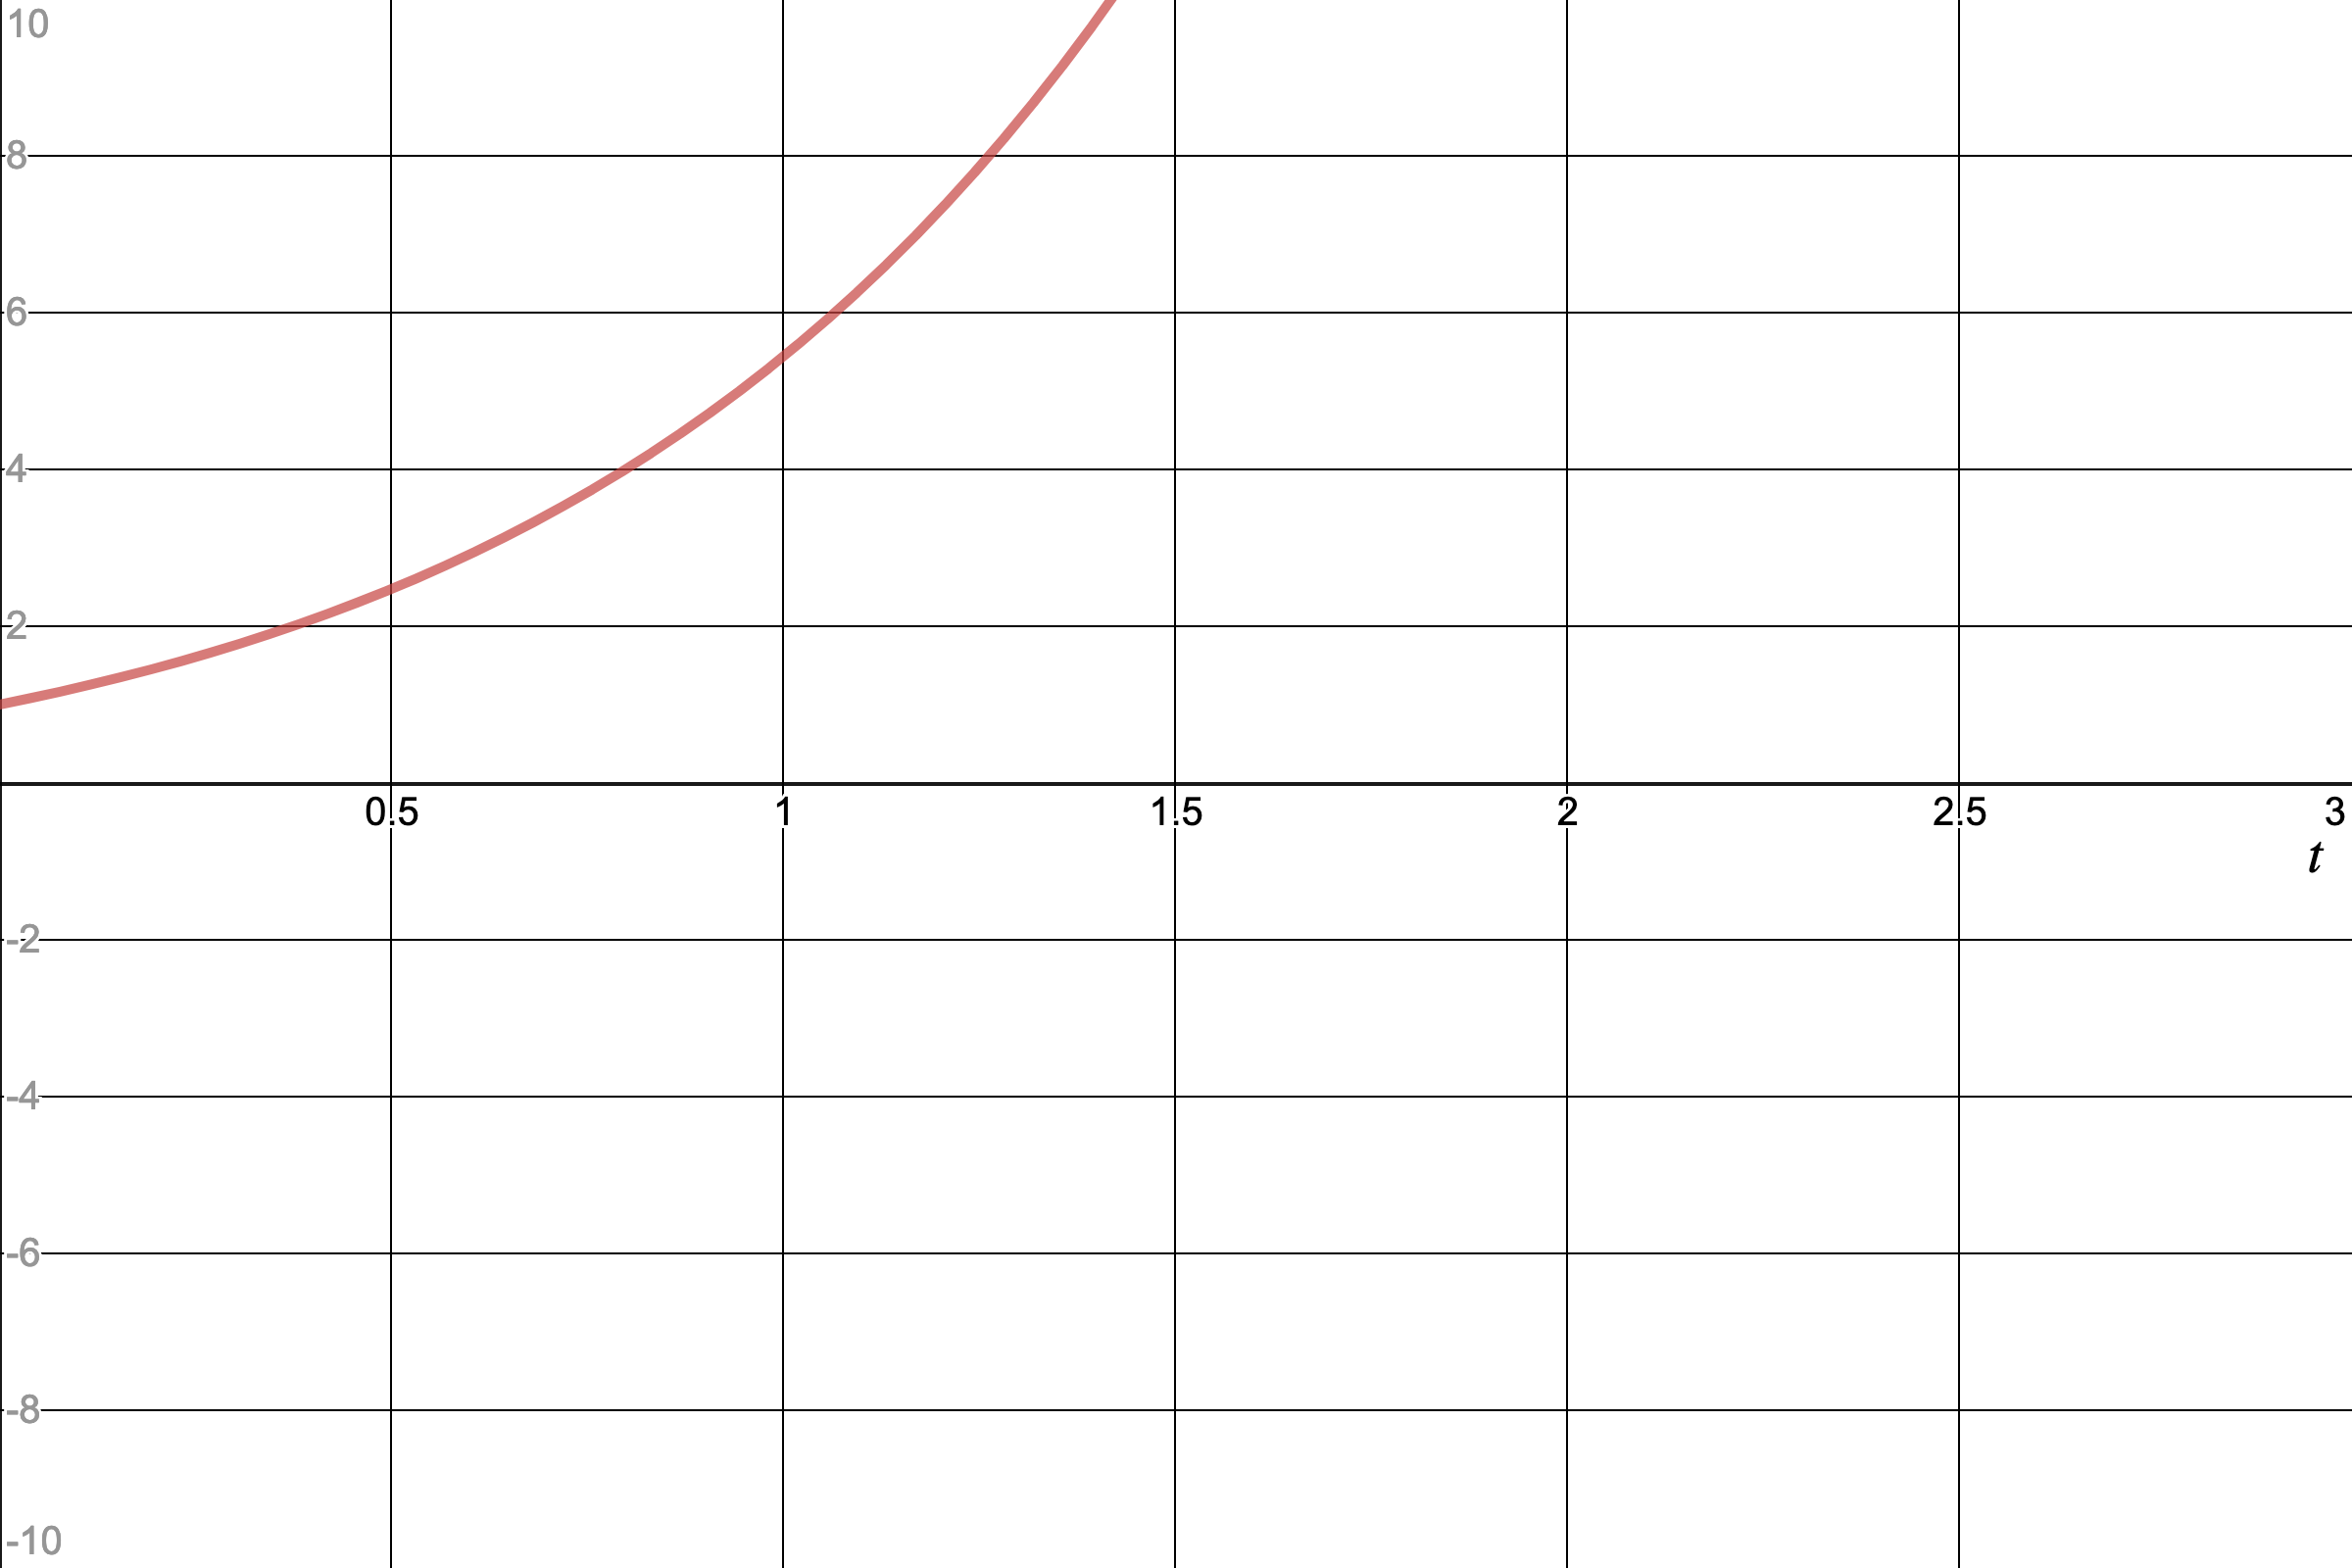
\includegraphics[width=.7\textwidth]{Figures_Part_2/l=1.png}
                \end{figure}
                We could also take $\lambda=-1$ with $C_1=C_2=1$ to see:
                \begin{figure}[H]
                    \centering
                    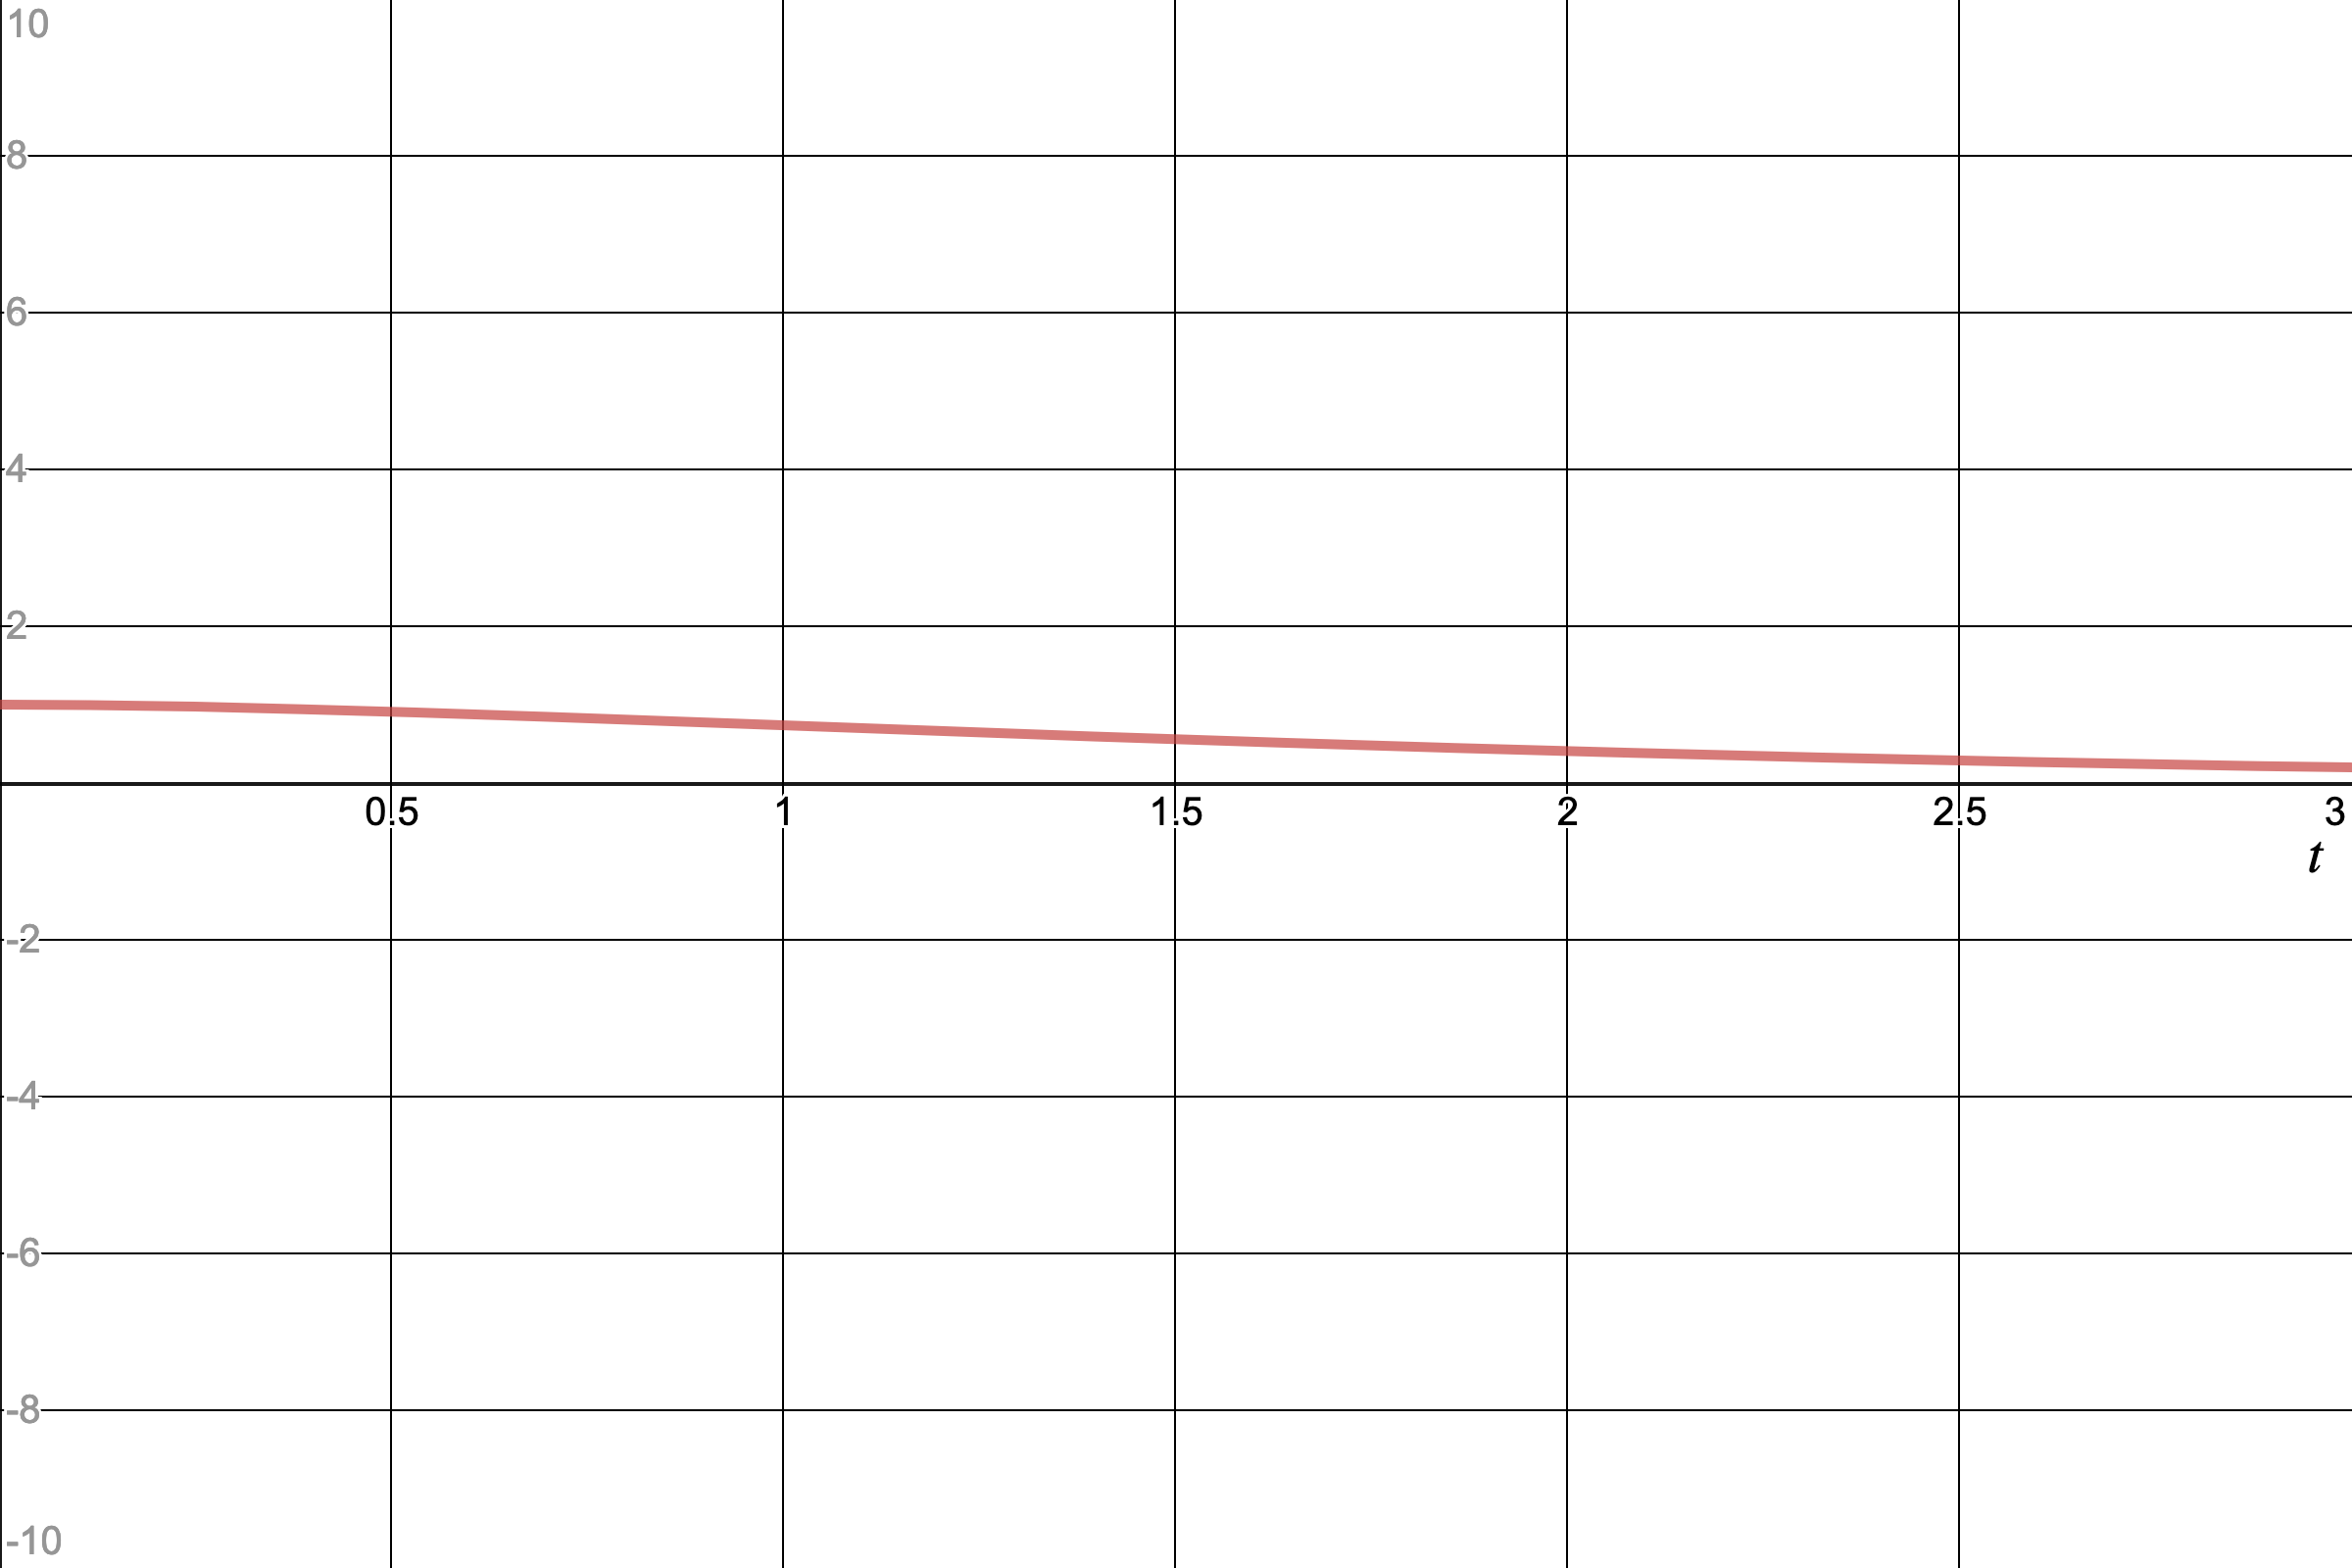
\includegraphics[width=.7\textwidth]{Figures_Part_2/l=-1.png}
                \end{figure}
            \end{itemize}
            \item \textbf{Case 2:} Consider the case where the roots to the characteristic polynomial are complex valued.  That happens when we have $b^2-4c$ since then we will have a square root of a negative number appear with the quadratic formula. In this case, if we have a root $\lambda$, then $\lambda^*$ is \underline{always} the other root (take a look at the quadratic formula, and see if you can see why this is the case).  Thus, we can put $\lambda=a+bi$ and then have another root $\lambda^*=a-bi$. This gives us the general solution
            \begin{align*}
                x(t)&= C_1 e^{\lambda t}+C_2 e^{\lambda^* t}\\
                &= C_1 e^{at}e^{ibt}+C_2e^{at}e^{-ibt}\\
                &= e^{at}\left( C_1 e^{ibt}+C_2 e^{-ibt}\right).
            \end{align*}
            Here, we must have that $C_1$ and $C_2$ are complex numbers.  We can also rewrite this general solution as
            \[
            x(t)= e^{at}(C_1 \cos(bt)+C_2\sin(bt)).
            \]
            
            Here we can take $a=1$ and $b=5$ with $C_1=C_2=1$ and plot the solution in the $xt$-plane to see:
            \begin{figure}[H]
                \centering
                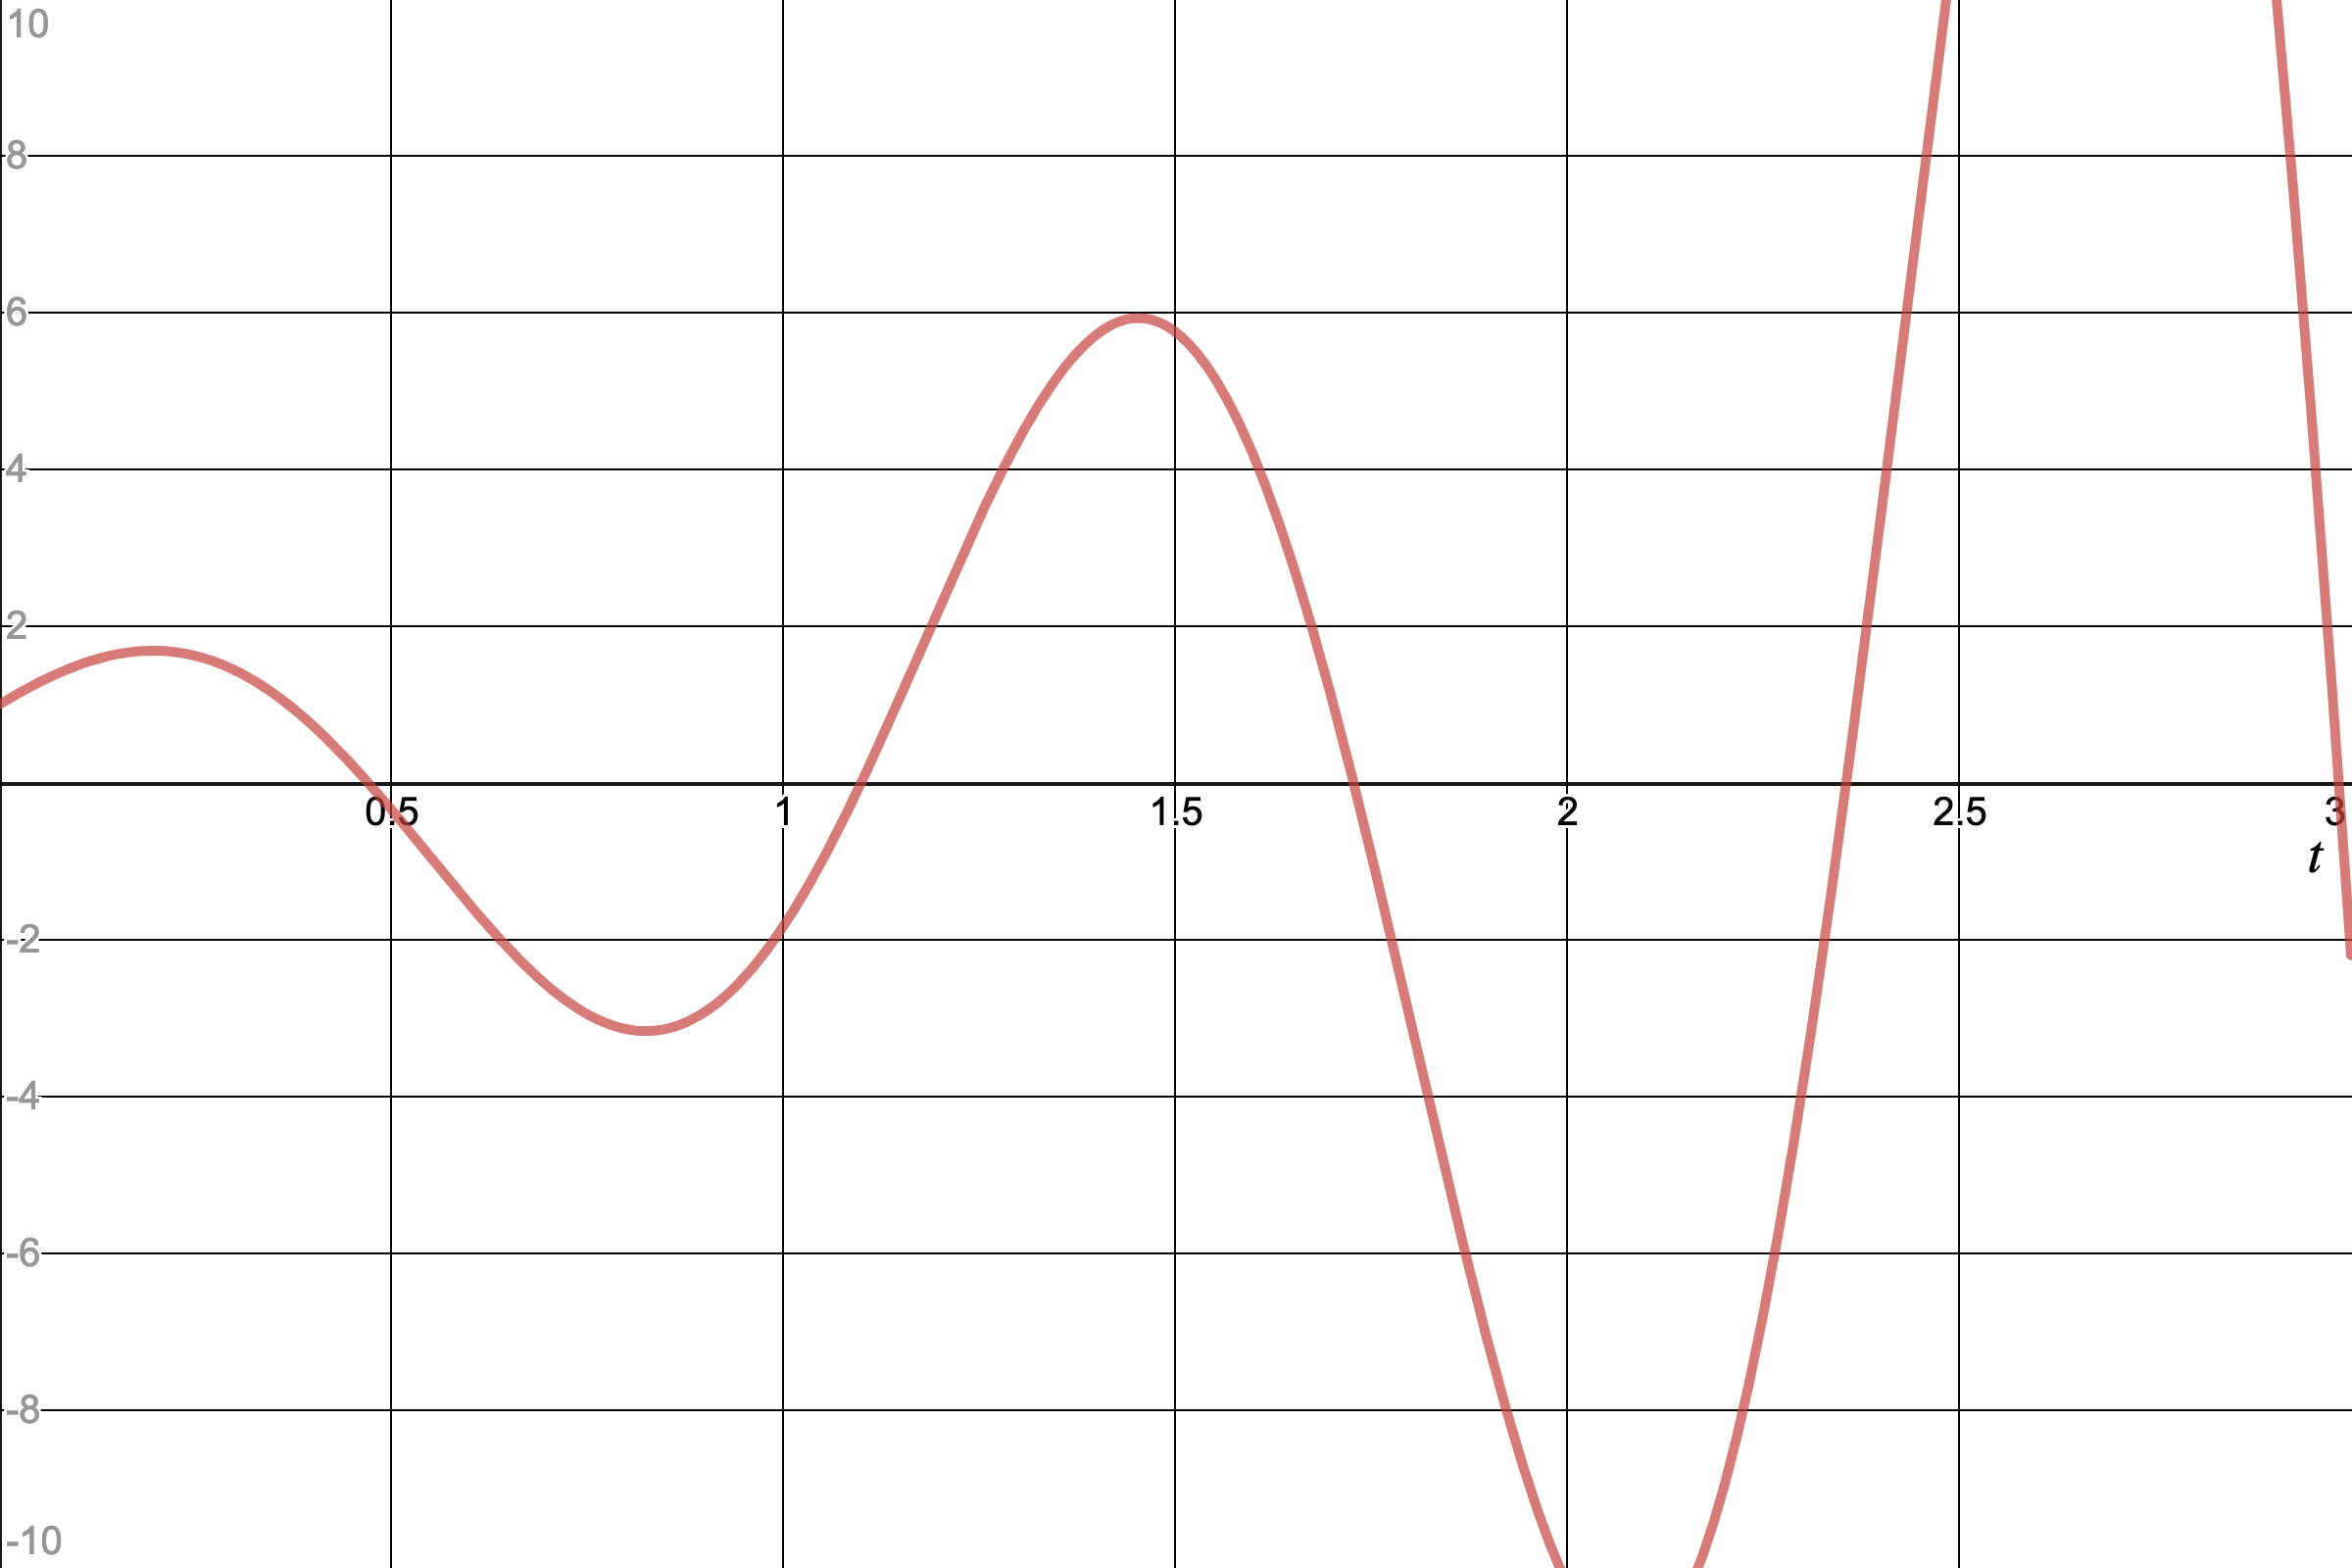
\includegraphics[width=.7\textwidth]{Figures_Part_2/a=1-b=5.png}
            \end{figure}
            We could also take the case with $a=0$, $b=5$, and $C_1=C_2=1$ and plot:
            \begin{figure}[H]
                \centering
                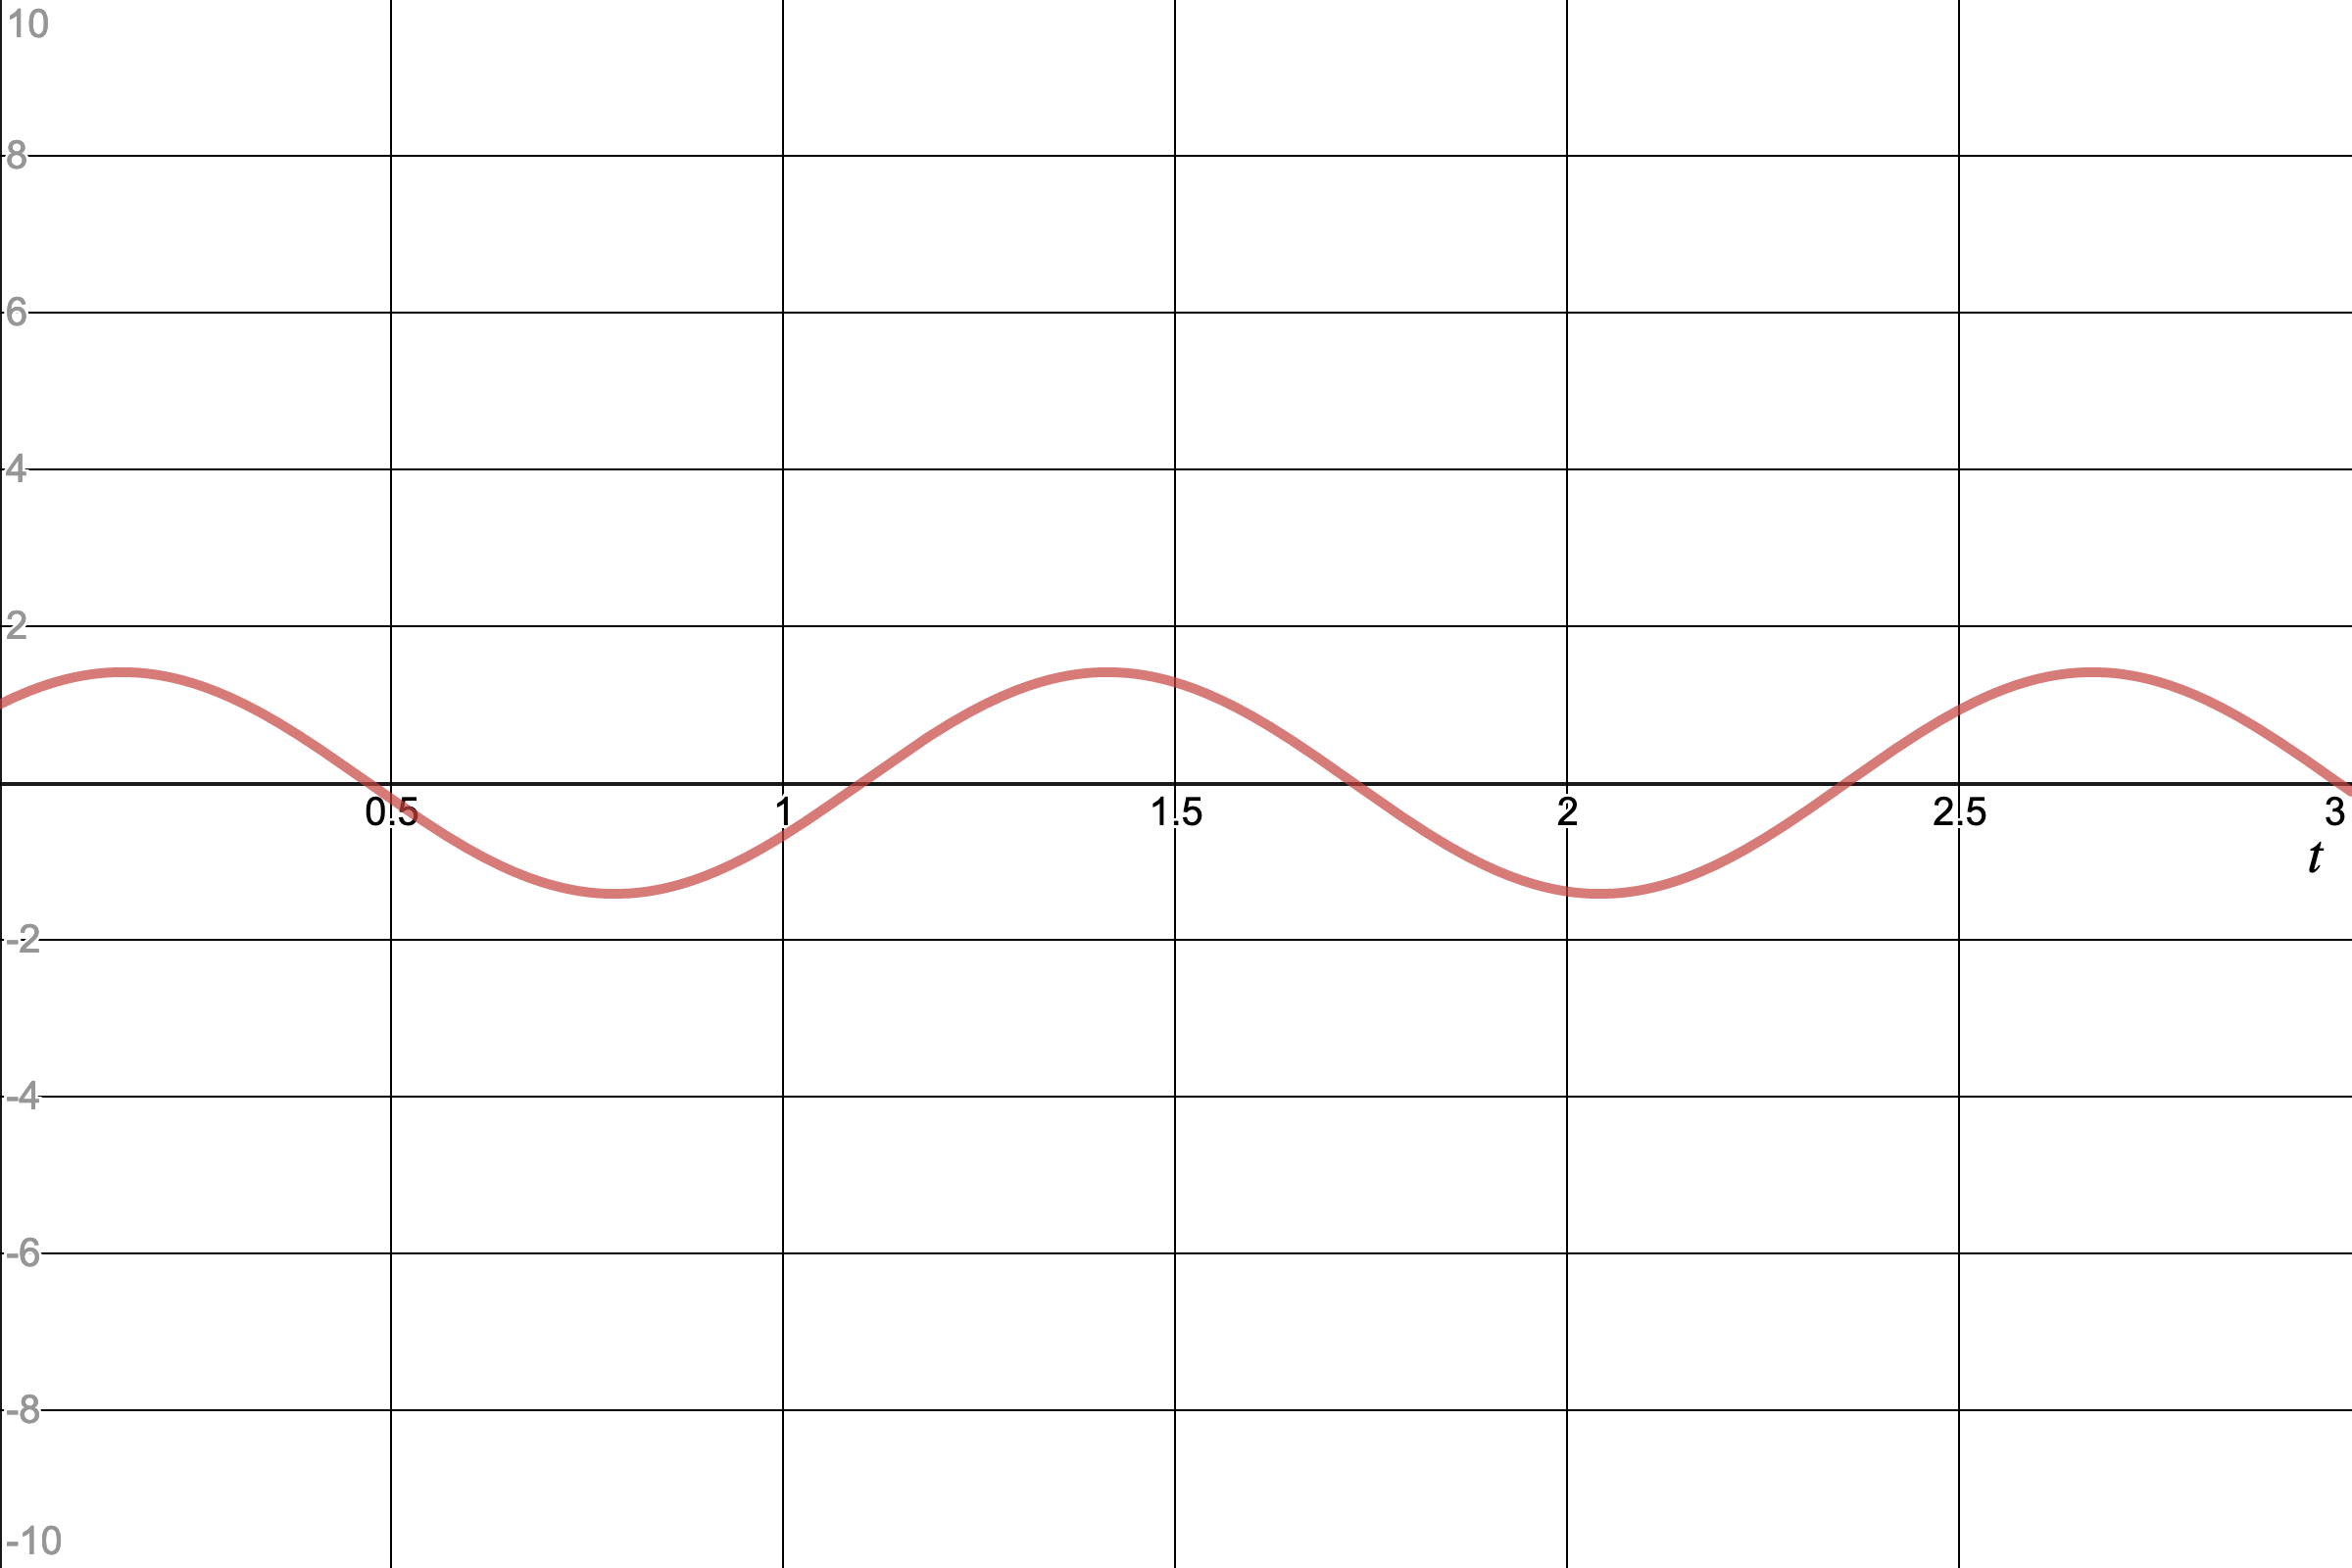
\includegraphics[width=.7\textwidth]{Figures_Part_2/a=0-b=5.png}
            \end{figure}
            Lastly, we could plot with $a=-1$, $b=5$ and $C_1=C_2=1$ to see:
                        \begin{figure}[H]
                \centering
                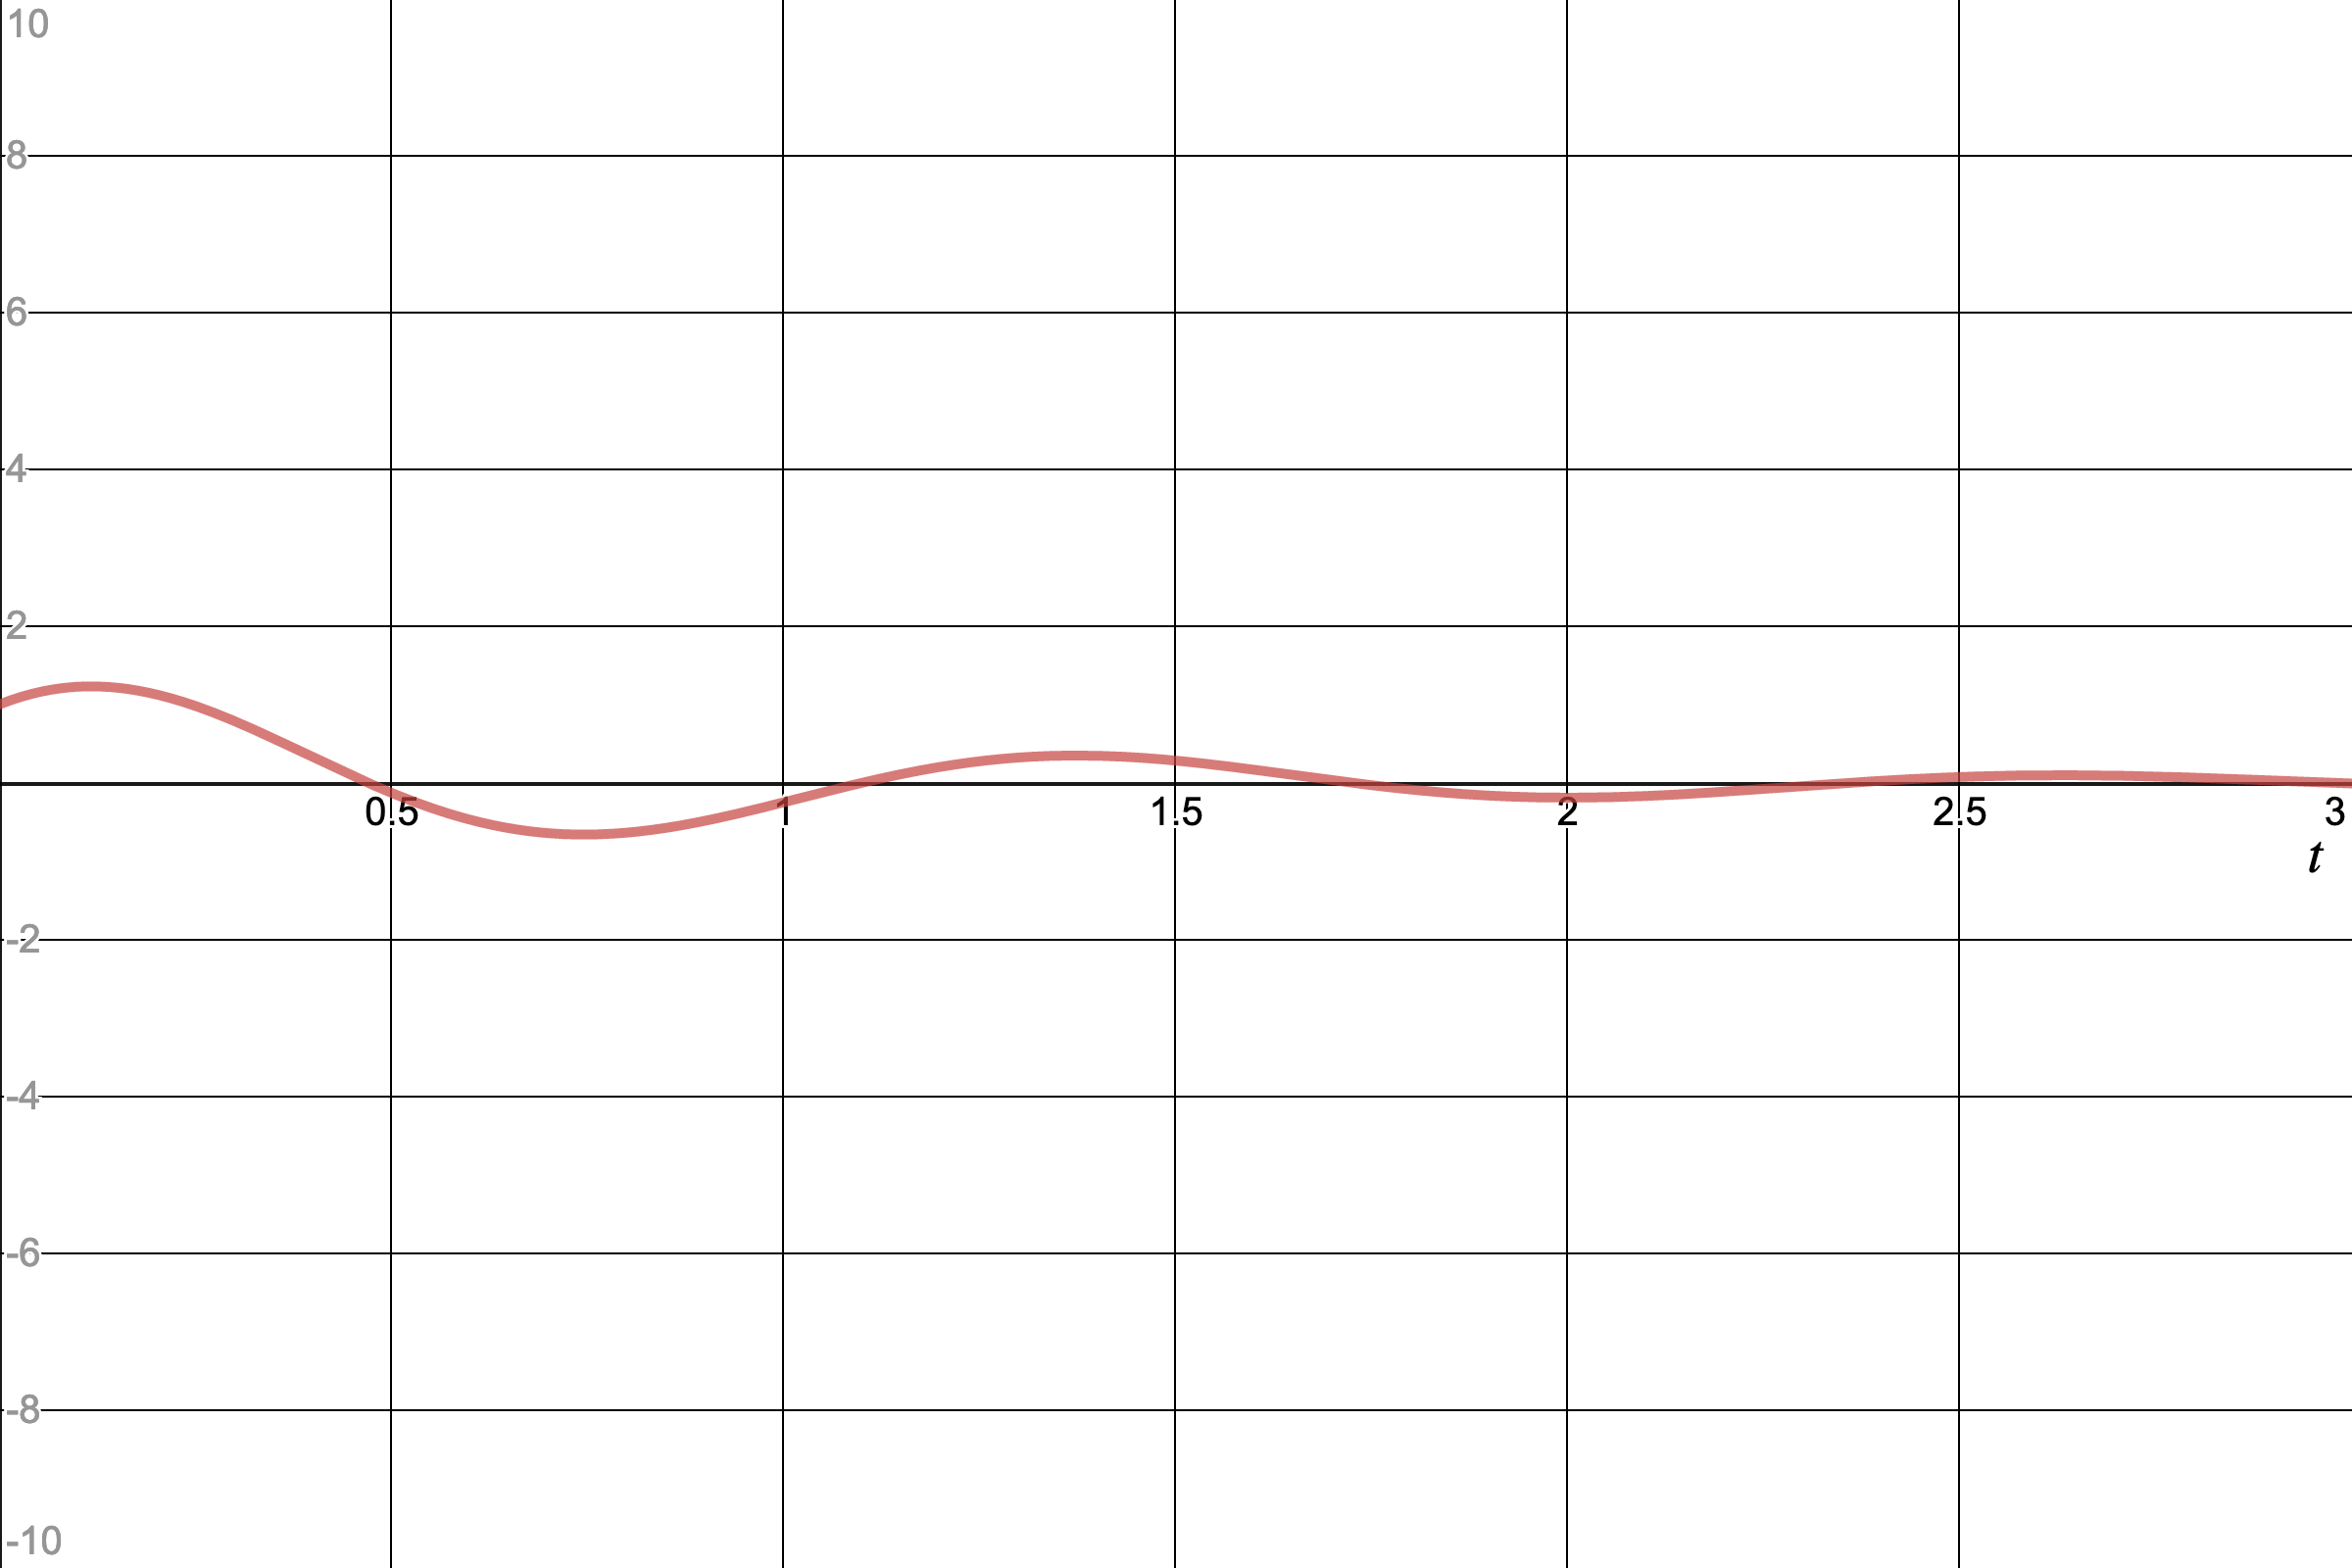
\includegraphics[width=.7\textwidth]{Figures_Part_2/a=-1-b=5.png}
            \end{figure}
        \end{itemize}
        
        \begin{exercise}
        Work out why if the roots to the characteristic polynomial are complex, that we always have the roots $\lambda$ and $\lambda^*$.
        \end{exercise}
        
        \begin{exercise}
        Show that the two general solutions
        \[
        x(t)=e^{at}(C_1 e^{ibt}+C_2e^{-ibt})
        \]
        and 
        \[
        x(t)=e^{at}(C_1 \cos(bt)+C_2\sin(bt))
        \]
        are equivalent using Euler's formula.
        \end{exercise}
        
        \subsection{Inhomogeneous Linear Equations}
        
        More often than not, we look at physical systems where there is some external force or potential that causes the system to change over time.  In the case of second order linear equations, this corresponds to the inhomogeneous equation
        \[
        x''+bx'+cx=F(t)
        \]
        where we think of $F(t)$ as an external force.  For specific forcing terms $F(t)$, we can solve this equation exactly using the \boldgreen{method of undetermined coefficients}\index{method of undetermined coefficients}.  The idea is that we can solve the homogeneous equation
        \[
        x_h''+bx_h'+cx_h=0
        \]
        to find a solution $x_h(t)$.  We refer to this as the \boldgreen{homogeneous solution}\index{homogeneous solution}. It does not, however, solve the equation on its own. We then need another function which we call the \boldgreen{particular integral}\index{particular integral} and denote by $x_p(t)$. This function is given by an ansatz based on what the forcing term is.  In this case, $x_p(t)$ solves the inhomogeneous equation
        \[
        x_p''+bx_p'+cx_p=F(t)
        \]
        but is needs to be accompanied by a homogeneous solution. The solution to an inhomogeneous equation as above will then be
        \[
        x=x_h+x_p.
        \]
        How do we know that this is a solution? We can check by taking
        \begin{align*}
            x''+bx'+cx&=(x_h+x_p)''+b(x_h+x_p)'+c(x_h+x_p)\\
            &= \underbrace{(x_h''+bx_h'+cx_h)}_{=0}+\underbrace{(x_p''+bx_p'+cx_p)}_{=F(t)}\\
            &=F(t).
        \end{align*}
        So the sum of a particular integral and a homogeneous solution is also a solution to the inhomogeneous equation! Now, let's see an example.
        
        \begin{ex}{Inhomogeneous Linear Equation with Constant Force}{inhom_linear}
        If we assume our equation has a quadratic forcing term $F(t)=2t^2$, then we have the equation
        \[
        x''+3x'+2x=2t^2.
        \]
        First, we find the solution to the homogeneous equation
        \[
        x_h''+3x_h'+2x_h=0
        \]
        which has the characteristic polynomial
        \[
        \lambda^2+3\lambda+2=0.
        \]
        The roots are then $\lambda_1=-1$ and $\lambda_2=-2.$ So we have that
        \[
        x_h(t)=C_1e^{-t}+C_2e^{-2t}.
        \]
        Next, we take an ansatz of $x_p(t)=a_0+a_1t+a_2t^2$ and call the $a_i$ coefficients the \boldgreen{undetermined coefficients}.  Then we have
        \[
        x_p'=a_1+2a_2t \qquad \textrm{and} \qquad x_p''=2a_2.
        \]
        We can plug these into our inhomogeneous equation
        \begin{align*}
        x''+3x'+2x&= 2a_2+3(a_1+2a_2t)+2(a_0+a_1t+a_2t^2)
        \end{align*}
        which we know should also be equal to the forcing term $F(t)$.  This gives us the equation
        \[
        2a_2+3(a_1+2a_2t)+2(a_0+a_1t+a_2t^2)=2t^2.
        \]
        We rearrange the terms as follows
        \[
        (2a_0+3a_1+2a_2)+(2a_1+6a_2)t+(2a_2)t^2=0+0t+2t^2
        \]
        which gives us the system of equations
        \begin{align*}
            2a_0+3a_1+2a_2&=0\\
            2a_1+6a_2&=0\\
            2a_2&=2.
        \end{align*}
        We can solve these to find $a_2=1$, $a_1=-3$ and $a_0=\frac{7}{2}$. So the particular integral is $x_p(t)=t^2-3t+\frac{7}{2}$.  Thus we have a solution
        \[
        x=x_h+x_p=C_1e^{-t}+C_2e^{-2t}+t^2-3t+\frac{7}{2}.
        \]
        If we were given initial data, we could solve for $C_1$ and $C_2$.
        \end{ex}
        
        
        \noindent Here's a table of the forms of $F(t)$ which will be solvable. You can use this to find an ansatz for the particular integral.  Once you know the ansatz it comes down to solving for the coefficients as we did in the previous example.
        \begin{table}[H]
        \centering
        \renewcommand{\arraystretch}{1.75}
            \begin{tabular}{c|c}
                Forcing Term $F(t)$&  Particular Integral $x_p$\\
                \hline
                $ke^{at}$ & $Ce^{at}$\\
                \hline
                $kt^n$ ~ $(n=0,1,2,\dots)$ & $\sum_{j=0}^n a_j t^j$\\
                \hline
                $k\cos(at)$ ~\textrm{or}~ $k\sin(at)$ & $K\cos(at)+M\sin(at)$\\
                \hline
                $ke^{at}\cos(bt)$ ~\textrm{or}~ $ke^{at}\sin(bt)$ & $e^{at}(K\cos(bt)+M\sin(bt))$\\
                \hline
                $\displaystyle{\left(\sum_{j=0}^n k_jt^j\right) \cos(bt)}$ ~\textrm{or}~ $\displaystyle{\left(\sum_{j=0}^n k_jt^j\right) \sin(bt)}$ & $\displaystyle{\sum_{j=0}^n\left( Q_jt^j \cos(bt) + R_jt^j \sin(bt)\right)}$\\
                \hline
                $\displaystyle{\left(\sum_{j=0}^n k_jt^j\right) e^{at}\cos(bt)}$ ~\textrm{or}~ $\displaystyle{\left(\sum_{j=0}^n k_jt^j\right) e^{at}\sin(bt)}$ & $\displaystyle{e^{at}\left(\sum_{j=0}^n \left( Q_jt^j \cos(bt) + R_jt^j \sin(bt)\right)\right)}$
            \end{tabular}
    \end{table}


        
        \newpage
        \section{Problems}
        \textcolor{blue}{to come}
        

        
